\chapter*{Глава 1. Многоногий шагающий аппарат c ортогональными движителями}
\addcontentsline{toc}{section}{Глава 1. Многоногий шагающий аппарат c ортогональными движителями}
В работе исследована кинематика многоногого шагающего аппарата с ортогональными движителями. Новизна такой кинематики состоит в уходе от использования природных кинематических схем ног, таких как нога насекомого или млекопитающего. Каждая нога обладает двумя поступательными взаимно перпендикулярными степенями свободы. В природе больше распространены вращательные соединения.

\begin{figure}[h]
\center{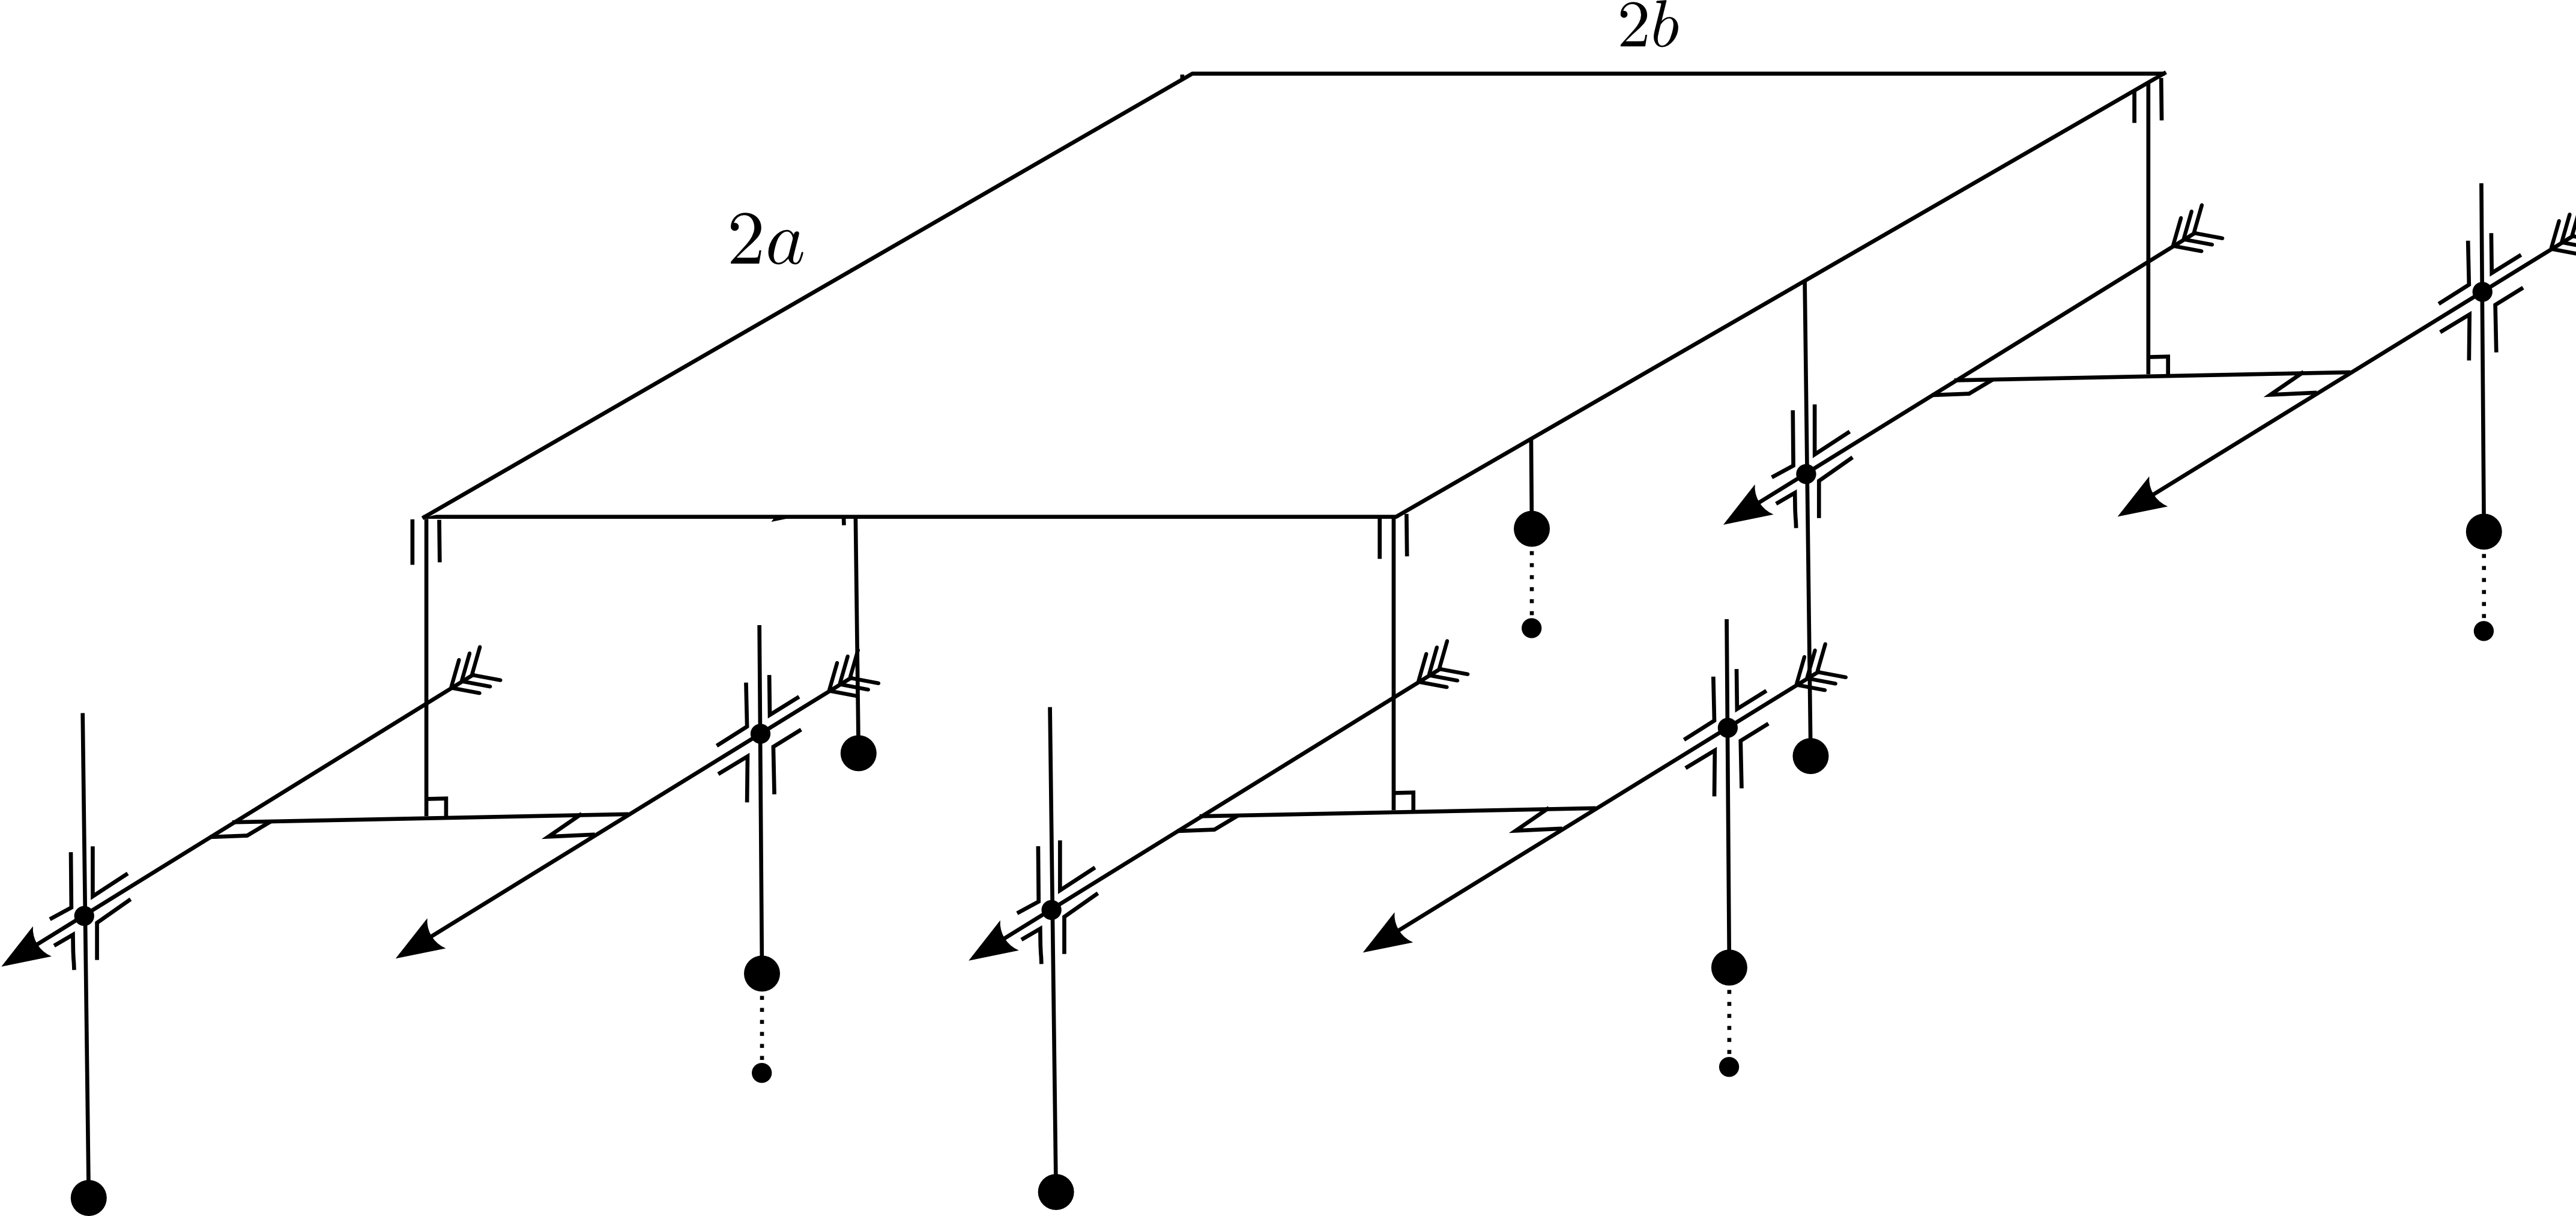
\includegraphics[width=100mm]{ortho_kinematics}}
\caption{Кинематическая схема аппарата}
\end{figure}

\section{Кинематическая схема аппарата}
Робот состоит из прямоугольного корпуса и четырех поворотных модулей. Поворотные модули будем называть H-модулями из-за сходства с русской буквой Н или латинской буквой H. Длина прямоугольного корпуса равна $2a$, ширина корпуса равна $2b$. Аппарат может перемещаться своим корпусом в горизонтальной плоскости $Oxy$. Положение корпуса задается координатами его центра $\overline{r}_c = (x,y)$ и углом поворота $\phi$ относительно неподвижной системы координат. В вершинах прямоугольника расположены шарнирные точки крепления поворотных модулей. Каждый Н-модуль состоит из двух ног c ортогональной кинематикой, расположенных в параллельных вертикальных плоскостях и симметрично отстоящих от оси вращения модуля на расстояние $c$. Пронумеруем поворотные модули при помощи индексов $(i,j)$: $i = 1$ - передний, $i = 2$ - задний; $j = 1$ - левый, $j = 2$ - правый.

\begin{figure}[h]
\center{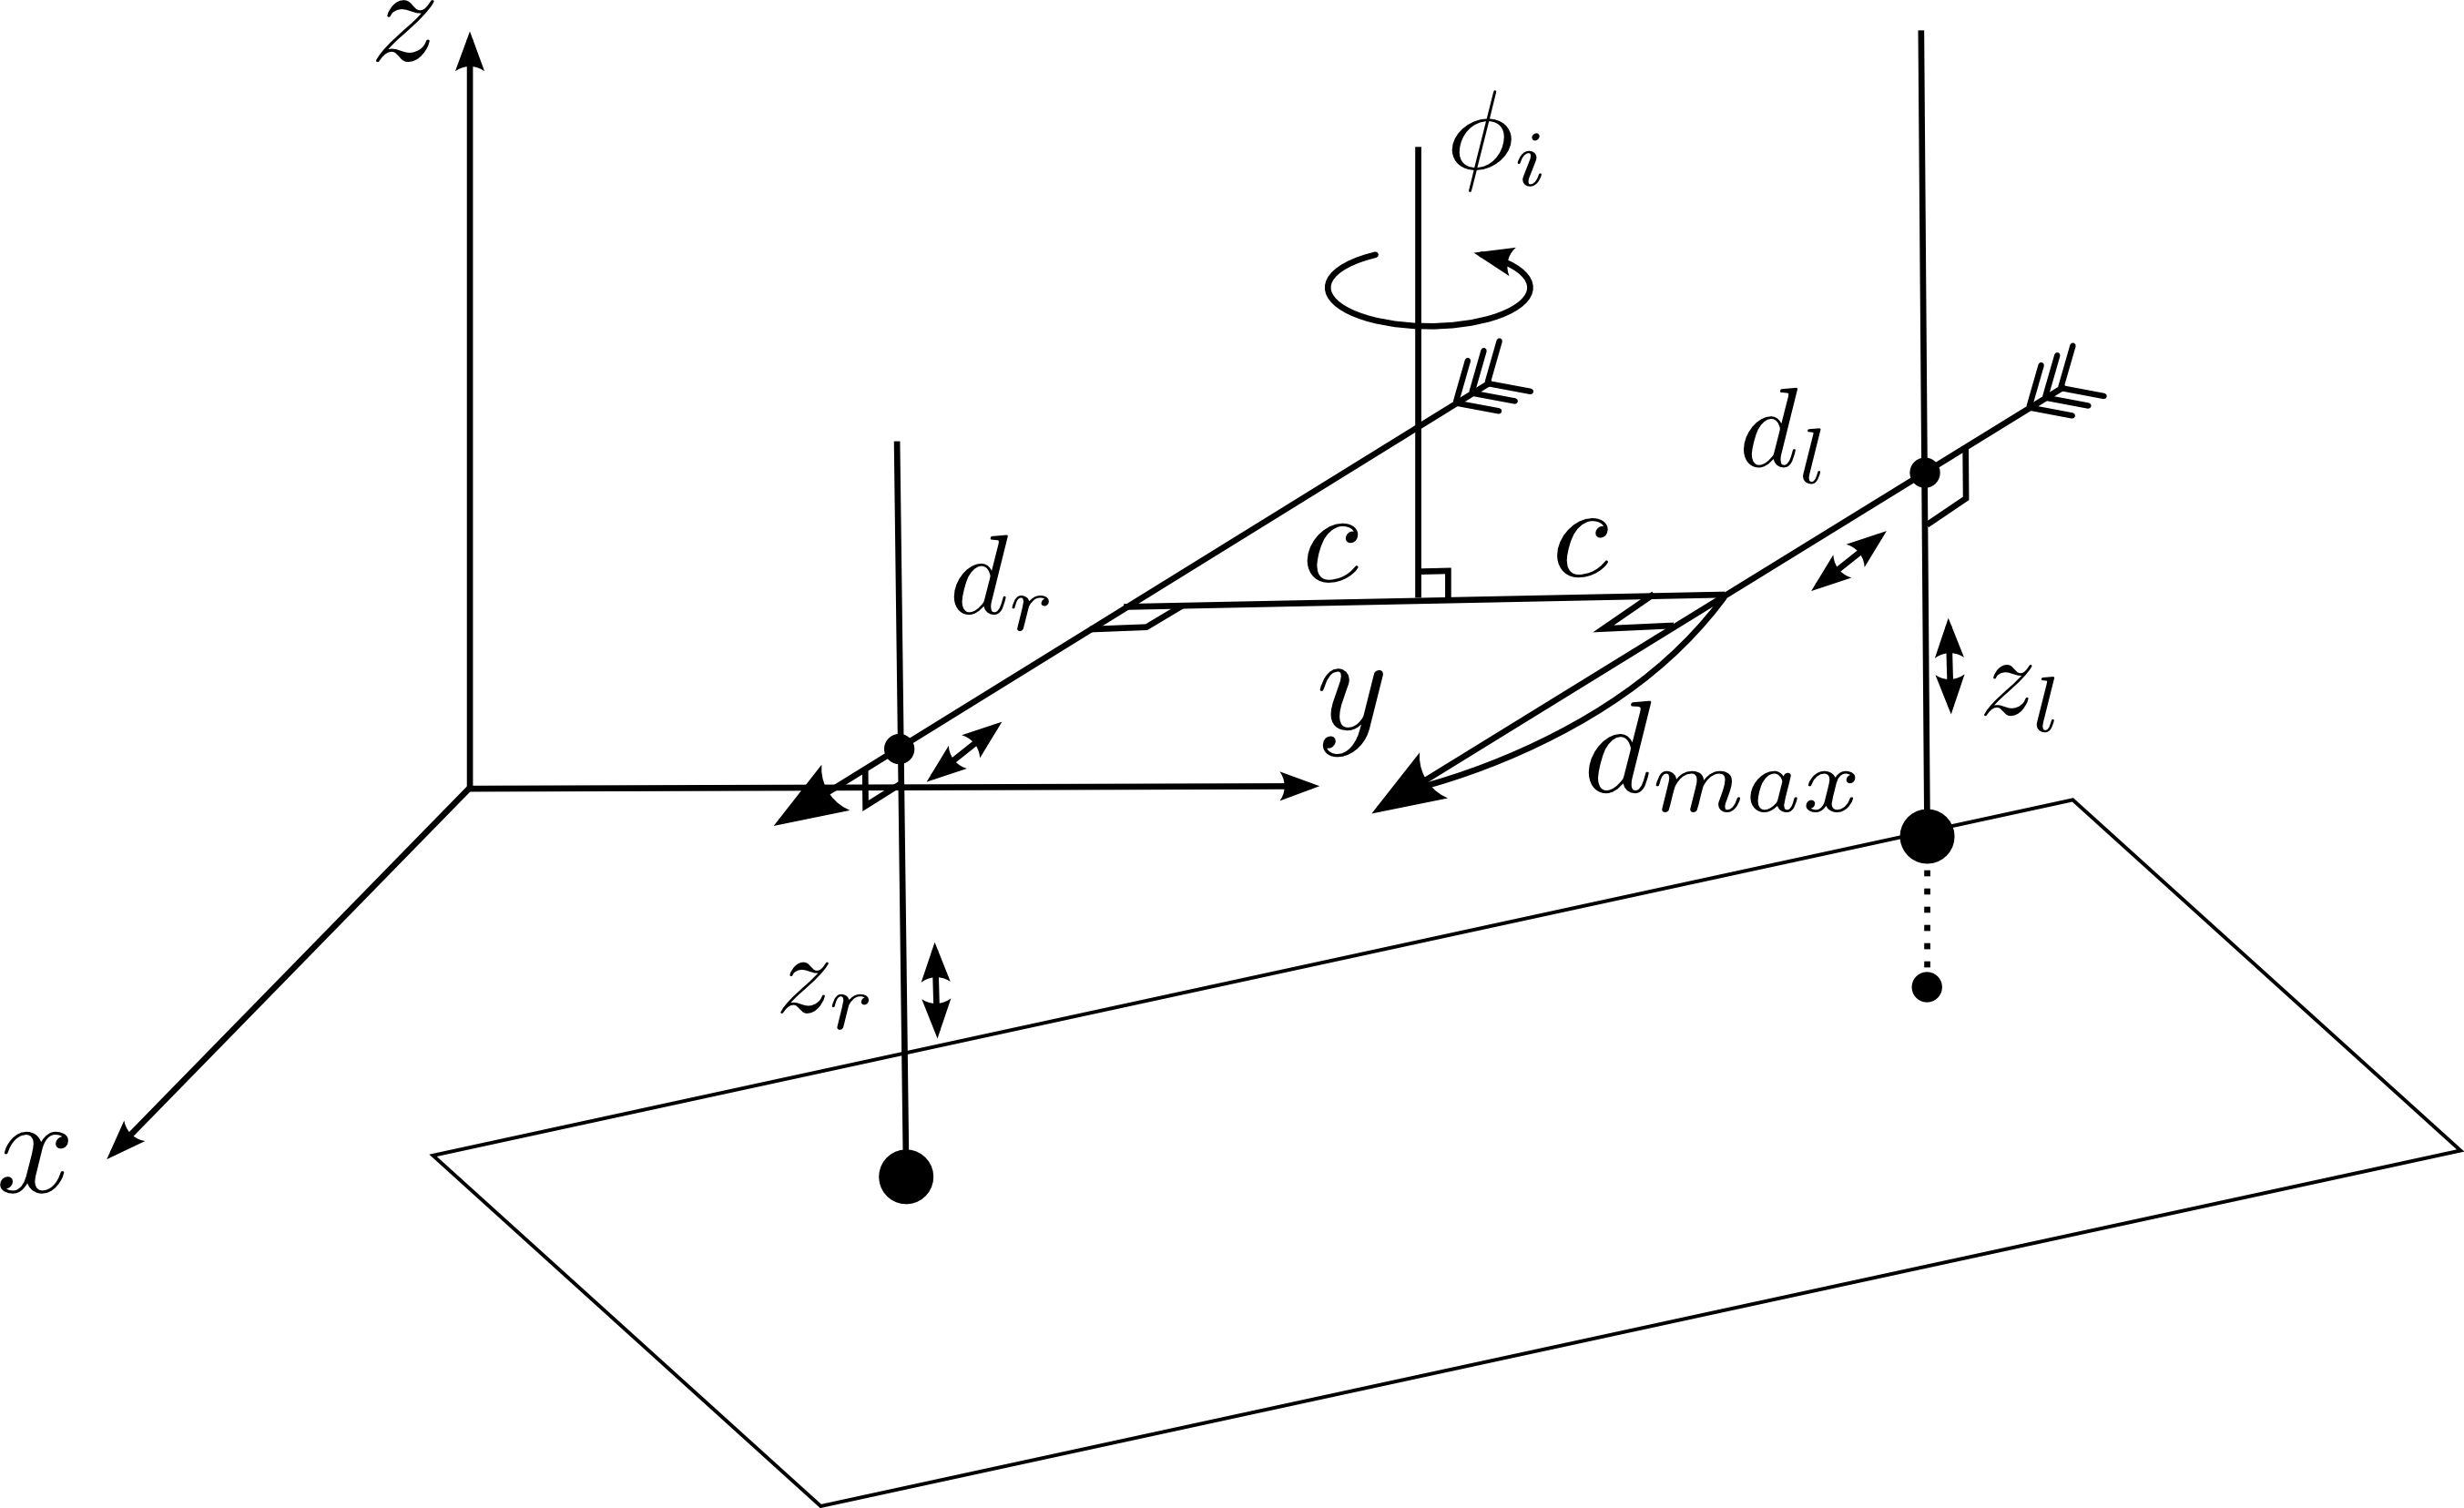
\includegraphics[width=100mm]{ortho_Hmodul}}
\caption{Кинематика Н-модуля}
\end{figure}

Координаты точек крепления поворотных модулей в абсолютной системе координат находятся из уравнений:

\begin{equation}
	\overline{r}_{ij} = \overline{r}_c+C(\phi)\left(
	\begin{array}{c}
	(-1)^{i+1}a\\
	(-1)^(j+1)b\\
	\end{array}\right)
\end{equation}

\subsection{Кинематика H-модуля}
Исследуем кинематику отдельного поворотного модуля. Кинематическая схема аппарата допускает независимое исследование кинематики каждого H-модуля в отдельности. Это следует из того, что по заданной для аппарата траектории $(x(t),y(t))$ и закону изменения его ориентации $\phi(t)$ однозначным образом строятся все траектории по которым перемещаются оси вращения H-модулей на плоскости $Oxy$. Из тех же соображений, синтез управления проводится для каждого модуля в отдельности с учетом согласования скоростей в точках крепления H-модулей к корпусу и расписанию перестановки ног для сохранения устойчивости аппарата.
Скорость точки крепления $\overline{V}_{ij}$ модуля $(i,j)$ находится из формулы Эйлера распределения скоростей в твердом теле:

\begin{equation}
\label{v_ij}
	\overline{V}_{ij} = \overline{V_c}+\overline{\omega}\,\times(\overline{r}_{ij}-\overline{r}_c),
\end{equation}

где $\overline{V_c} = \left(\begin{array}{c}\dot{x}\\\dot{y}\\\end{array}\right)$ это скорость центра аппарата на заданной траектории, $\overline\omega =(0,0,\dot\phi)^T$ - угловая скорость корпуса, $(\overline{r}_{ij}-\overline{r}_c)$ - радиус-вектор от центра корпуса до оси H-модуля с индексом $(i,j)$.

\subsection{Прямая кинематическая задача}
Конфигурация Н-модуля на плоскости определяется семью параметрами. Радиус вектор $ \overline{r}_{ij} = (x_{ij},y_{ij})^T$ определяет координаты оси вращения H-модуля на плоскости $Oxy$,$\theta_{ij}$ - абсолютный угол поворота Н-модуля в неподвижной системе координат, набор чисел $(d^l_{ij},d^r_{ij},z^l_{ij},z^r_{ij})$ определяют конфигурацию ног модуля. Параметры $2\,c$  и $2\,d_{max}$ задают соответственно ширину и длину H-модуля. Считаем, что для координат $(d^l_{ij},d^r_{ij})$ выполнено условие:

\begin{equation}
	\label{d_constraint}
	|d^k_{ij}|\leq d_{max},k = l,r.
\end{equation}

В каждый момент времени только одна нога модуля находится в опорной фазе и не будем подробно останавливаться на исследовании координат $z_l$ и $z_r$.

Пусть точка $\overline{r}^o_{ij} = (x^o_{ij},y^o_{ij})^T$ является опорной для левой ноги модуля. Тогда в системе координат связанной с H-модулем точка $\overline{r}^o_{ij}$ имеет координаты $(d^l_{ij},c)$ и верна следующая система уравнений:

	\begin{equation}
	\label{kinematics}
	\left\{
	\begin{array}{lcr}
	x^o_{ij} = x_{ij} + d^l_{ij}\,cos(\phi_{ij})-c\,sin(\phi_{ij})\\
	y^o_{ij} = y_{ij} + d^l_{ij}\,sin(\phi_{ij})+c\,cos(\phi_{ij})\\
	\end{array}
	\right.
	\end{equation}
	или в векторной форме
	\begin{equation}
	\label{kinematics_vector}
	\overline{r}^o_{ij} = \overline{r}_{ij}+ C(\phi_{ij})\,
	\left(
	\begin{array}{lll}
	d^l_{ij}\\
	c\\
	\end{array}
	\right),
	\end{equation}
	где $C(\phi_{ij})$ это матрица поворота на угол $\phi_{ij}$ вокруг вертикальной оси.\\
	
\subsection{Обратная кинематическая задача}
Исследуем обратную кинематическую задачу. По заданным координатам опорной точки в абсолютной системе координат и известному положению центра модуля восстановим значения координат $(d^l_{ij},\phi^l_{ij})$.

Обращая систему (\ref{kinematics}) без учета ограничения (\ref{d_constraint}) , получаем четыре возможных варианта ответа:
	\begin{equation}\label{revkin}
	\left\{
	\begin{array}{lcr}
	d^l_{ij} = \pm\sqrt{(x^o_{ij}-x_{ij})^2+(y^o_{ij}-y_{ij})^2-c^2}\\
	\phi^l_{ij}  = arctg\left(\dfrac{y^o_{ij}-y_{ij}}{x^o_{ij}-x_{ij}}\right) \pm arccos\left(\dfrac{d^l_{ij}}{\sqrt{c^2+{d^l_{ij}}^2}}\right)\\ 
	\end{array}
	\right.
	\end{equation}
	
В зависимости от выбора знака $d^l_{ij}$ для каждой ноги модуля возможны два варианта решения обратной задачи. Можно заметить, что уравнения (\ref{revkin}) подходят и для решения обратной кинематической задачи для правой ноги поворотного модуля. Значения для $d^r_{ij}$ совпадают со значениями $d^l_{ij}$, а для угла ориентации Н-модуля будет верно: 


\begin{equation}
\phi^r_{ij} = arctg\left(\dfrac{y^o_{ij}-y_{ij}}{x^o_{ij}-x_{ij}}\right) \mp arccos\left(\dfrac{d^r_{ij}}{\sqrt{c^2+{d^r_{ij}}^2}}\right)
\end{equation}

Для Н-модуля в совокупности существует 4 способа постановки ноги в заданную опорную точку.


\subsection{Влияние кинематических ограничений}
Реальные исполнительные механизмы обладают рядом физических ограничений на возможные положения и допустимые скорости и ускорения. Исследуем влияние ограничений по скорости на кинематику аппарата.
В первую очередь интересны ограничение на максимальную угловую скорость $(\dot{\phi}_{ij}-\dot{\phi})$ поворота Н-модуля относительно корпуса аппарата и ограничение на максимальную скорость переноса ноги $\dot{d}^k_{ij}$:

\begin{equation}\label{limitations}
	|\dot{\phi}_{ij}-\dot{\phi}| \leq \omega_{max},\quad|\dot{d}^k_{ij}|\leq \dot{d}_{max}
\end{equation}


Продифференцируем уравнения (\ref{kinematics_vector}) по времени:

\begin{equation}
\label{kinematics_diff}
0 = \overline{V}_{ij}+\dot{\phi_{ij}}\dfrac{\partial{C(\phi_{ij})}}{\partial(\phi_{ij})}
	\left(\begin{array}{c}
	d^l_{ij}\\
	c\\
	\end{array}\right)
	+C(\phi_{ij})\left(\begin{array}{c}
	\dot{d}^l_{ij}\\
	0\\
	\end{array}\right)
\end{equation}

Обращая систему (\ref{kinematics_vector}) получаем систему уравнений:

\begin{equation}
\label{kinematics_solved}
\left\{
\begin{array}{rcl}
	d^l_{ij}\dot{\phi}_{ij} & = & \dot{x}_{ij}\,sin(\phi_{ij}) - \dot{y}_{ij}\,cos(\phi_{ij})\\
	\\
	\dot{d}^l_{ij} & = & -(\dot{x}_{ij}\,cos(\phi_{ij})+\dot{y}_{ij}\,sin(\phi_{ij}))+c\,\dot{\phi}_{ij}\\
\end{array}\right.
\end{equation}

При $d^l_{ij}\ne 0$ получаем выражения для $\phi_{ij}$ и $\dot{d}^l_{ij}$:
	\begin{equation}\label{soldotphiandd}
	\left\{
	\begin{array}{lcr}
	\dot{\phi_{ij}} = \dfrac{(\dot{x}_{ij}\,sin(\phi_{ij}))-\dot{y}_{ij}\,cos(\phi_{ij})}{d^l_{ij}}\\
	\dot{d}^l_{ij} = c\,\dot{\phi_{ij}}-(\dot{x}_{ij}\,cos(\phi_{ij})+\dot{y}_{ij}\,sin(\phi_{ij}))\\
	\end{array}
	\right.
	\end{equation}
Подставим выражения~(\ref{soldotphiandd}) в неравенства~(\ref{limitations}) и введем новые переменные $(V,t)\mapsto(\dot{x}_{ij},\dot{y}_{ij}):$

	\begin{equation}
	\label{substitution}
	\left\{
	\begin{array}{lcr}
	\dot{x_{ij}} = V_{ij}\,cos(\gamma_{ij})\\
	\dot{y_{ij}} = V_{ij}\,sin(\gamma_{ij})\\
	\end{array}
	\right.
	, V \geq 0 , \gamma_{ij}\in(-\pi;\pi],
	\end{equation}
	
и обозначим $\delta_i:=(\gamma_{ij}-\phi_{ij})$. Угол $\delta_{ij}$ задает направление вектора скорости оси Н-модуля в системе координат связанной с Н-модулем. После замены переменных получаем неравенства:
	\begin{equation}
	\label{limitations_subsed}
	\begin{array}{lcr}
	\left|\dfrac{-V_{ij}}{d^l_{ij}}\,sin(\delta_{ij})-\dot{\phi}\right|\leq{w_{max}},\\
	\\
	\left|\dfrac{c\,V_{ij}}{d^l_{ij}}sin(\delta_{ij})-V_{ij}\,cos(\delta_{ij})\right|\leq{\dot{d}_{max}}.\\
	\end{array}
	\end{equation}
	
При помощи неравенств (\ref{limitations_subsed}) можно выполнять проверку корректности задания параметризации движения корпуса аппарата по траектории. По заданным $(x(t),y(t),\phi(t))$ можно найти скорости осей всех Н-модулей и проверить, что для данного маневра с данным набором опорных точек не будет превышения по допустимым скоростям поступательных и поворотных приводов в каждом Н-модуле. Совместное решение неравенств (\ref{limitations_subsed}) относительно $V_{ij}$ для каждого модуля позволяет найти максимальную возможную скорость $\overline{V}_c$ аппарата на заданной траектории. Можно заметить, что при выводе неравенств (\ref{limitations_subsed}) никак не использовался тот факт, что опорной была левая нога. 

Рассмотрим пару случаев значения угла $\delta_{ij}$ направления скорости оси Н-модуля. Пусть $\delta_{ij} = \pi\,k,k\in \mathbb{Z}$ - соответствует случаю, когда скорость точки крепления Н-модуля направлена строго вдоль поворотного модуля. В данном случае неравенства (\ref{limitations_subsed}) принимают следующий вид:

\begin{equation}
\begin{array}{rcl}
|\dot{\phi}|&\leq&\omega_{max}\\
\\
|V_{ij}|&\leq&\dot{d}_{max}\\
\end{array}
\end{equation}

Абсолютная угловая скорость Н-модуля в данном случая равна нулю, работает только поступательная координата.

Пусть значение $\delta_{ij} = \dfrac{\pi}{2}+\pi\,m, m \in \mathbb{Z}$ - соответствует случаю, когда вектор скорости точки крепления поворотного модуля направлен строго поперек модуля. В данном случае, ограничения (\ref{limitations_subsed}) принимают вид:

\begin{equation}
\begin{array}{rcl}
|\dfrac{-V_{ij}}{d^l_{ij}}-\dot{\phi}|&\leq&\omega_{max}\\
\\
|\dfrac{c\,V_{ij}}{d^l_{ij}}|&\leq&\dot{d}_{max}\\
\end{array}
\end{equation}

Осталось рассмотреть случай $d^l_{ij}=0$. Второе уравнение системы (\ref{kinematics_solved}) принимает вид:

\begin{equation}
0 = \dot{x}_{ij}\,sin(\phi_{ij})-\dot{y}_{ij}\,cos(\phi_{ij}) + 0\,\dot{\phi}_{ij}
\end{equation}
	
	Применяя замену (\ref{substitution}) получаем:
	
	\begin{equation}
		0 = V\,sin(\delta_{ij})
	\end{equation}
	
	Проекция скорости точки крепления Н-модуля на поперечную ось поворотного модуля всегда равна нулю. Это значит что первое уравнение системы (\ref{kinematics_solved}) принимает вид:
	
	\begin{equation}
		\dot{d}^l_{ij} = -|V_{ij}|+c\,\dot{\phi_{ij}}
	\end{equation}
	
Неравенства (\ref{limitations_subsed}) примут вид:

\begin{equation}
\begin{array}{rcl}
|\dot{\phi}_{ij}-\dot{\phi}|&\leq&\omega_{max}\\
\\
|\dot{d}^l_{ij} = -|V_{ij}|+c\,\dot{\phi}_{ij}|&\leq&\dot{d}_{max}\\
\end{array}
\end{equation}

%%Достаточно рассмотреть случай, когда выражения, стоящие под знаком модуля, положительны.
%%	\begin{equation}\label{limitswithsubs}
%%	\begin{array}{lcr}
%%	V\leq\dfrac{d_i\,\omega_{max}}{sin(\delta_i)}\\
%%	V\leq\dfrac{d^i_{max}\,d}{c\,sin(\delta_i)+d_i\,cos(\delta_i)}\\
%%	\end{array}
%%	\end{equation}
%%Угол $\delta_i$ определяет направление скорости перемещения оси H-модуля в подвижной системе координат, а $V$ абсолютную величину скорости. Нам требуется определить максимальную допустимую величину $V$.
%%Построим поверхность $V = \dfrac{d_i\,\omega_{max}}{sin(\delta_i)}$ (рис. \ref{Vsurf})для первого неравенства из ~(\ref{limitswithsubs}):
%%
%%\begin{figure}[h]
%%\center{\includegraphics[width = 100mm]{dotphi}}
%%\caption{Зависимость скорости $V$ от $d_i$ и $\delta$ }
%%\label{Vsurf}
%%\end{figure}
%%
%%\begin{figure}[h]
%%\center{\includegraphics[width = 100mm]{dotphicontour}}
%%\caption{Сечение поверхности (рис. \ref{Vsurf}) плоскостями $d_i = const$}
%%\label{dotphicontour}
%%\end{figure}
%%
%%При каждом фиксированном значении $d_i$ имеем сечение полученной поверхности (\ref{dotphicontour}).
%%Значения $\delta = \pm \dfrac{\pi}{2}$ являются экстремальными. В этих точках $V_{max} = \omega_{max}\,d_i$.
%%На практике это значит, что если скорость $V$ H-модуля направлена под углом $\pm\dfrac{\pi}{2}$ к углу его ориентации $\phi_i$, то модулю нельзя двигаться по своей траектории со скоростью большей, чем $V_{max} = \omega_{max}\,d_i$.

\section{Синтез движений аппарата}
Движение аппарата будет строится при помощи маневров разворота вокруг неподвижного центра корпуса аппарата и поступательных перемещений аппарата вдоль прямолинейных отрезков. Вся траектория движения робота разбивается на цепочку прямолинейных отрезков, а в вершинах полученной ломанной аппарат выполняет развороты на месте на заданный угол.

\subsection{Поступательное движение аппарата}
Рассмотрим движение H-модуля в окрестности своей опорной точки. Значения его поступательной и угловой координаты определяются соотношением (\ref{revkin}). Из выражения для $d^l_{ij}$ следует, что минимум этой функции достигается на окружности с центром в точке$(x^o_{ij},y^o_{ij})$ и радиусом $c$. На этой окружности $d^l_{ij} = d^l_{ij}(x,y) = 0$. Если траектория движения оси Н-модуля не касается данной окружности, то минимум значения функции $d(x,y)$ будет строго положителен или строго отрицателен, в зависимости от того на какой половине поступательной степени находился образ опорной точки в начальный момент движения. Если траектория проходит через внутренность окрестности опорной точки, то в этой области не определена функция $d^l_{ij}(x,y)$ и решения не существует, т.е. ось Н-модуля не сможет выполнить данное движение. Это следует из того, что плечо $c$, на которое отстоит плоскость ноги от оси вращения модуля, величина постоянная и отличная от нуля и ось Н-модуля не сможет приблизиться к опорной точке ближе чем на расстояние равное $c$. Переход через точку $d = 0$ возможен только если траектория оси поворотного модуля касается или лежит на окружности радиуса $c$ с центром в опорной точке.

С технической точки зрения, переход через положение $d^l_{ij}=0$ означает, что переносная степень используется более эффективно. Это дает больший шаг и делает более равномерным износ деталей механизма.
По заданной траектории H-модуля определим геометрическое множество возможных опорных точек. В каждой точке траектории $(x(t),y(t))$ построим нормаль и отложим расстояние $\pm c$. Полученные кривые будут геометрическим местом возможных опорных точек для левой и правой ноги H-модуля. Такой тип кривых называется эквидистантами.

Рассмотрим поступательное движение корпуса аппарата по прямой траектории. Все траектории движения точек крепления Н-модулей параллельные прямые. Эквидистантами к траекториям точек крепления Н-модулей так же являются параллельные прямые. В случае прямолинейного движения и выборе опорных точек на эквидистантах, поступательная степень сможет изменяется в интервале $[-d_{max},d_{max}]$, углы ориентации Н-модулей $\phi_{ij}$ ,будут постоянны и их производные будут равны нулю, временное расписание перестановки ног выбирается таким образом, чтобы обеспечить статическую устойчивость аппарата в каждый момент времени.

\subsection{Поворот на месте}
Рассмотрим поворот аппарата вокруг геометрического центра корпуса. Пусть в начальный момент корпус аппарата имеет ориентацию $\phi=0$, центр корпуса располагается в начале системы координат $Oxy$, все H-модули выстроены вдоль корпуса аппарата, т.е. все $\phi_{ij}(t = 0)=0$. В такой конфигурации аппарат находится после поступательного движения вдоль прямолинейного отрезка пути. Требуется совершить маневр при котором корпус аппарата повернется вокруг своего геометрического центра на любой заданный угол так, чтобы в конечном положении все H-модули были так же ориентированы вдоль корпуса аппарата, чтобы аппарат смог продолжить движение вдоль следующего прямолинейного участка траектории.

\begin{figure}[h]
\center{\includegraphics[width=80mm]{ortho_2013_rotation}}
\caption{Поворот аппарата на заданный угол}
\end{figure}

При развороте вокруг центра корпуса, все точки крепления H-модулей лежат на одной окружности радиуса $R = \sqrt{a^2+b^2}$, где $2\,a - $длина, а $2\,b - $ширина корпуса аппарата. Аппарат совершает поворот вокруг своего центра, поэтому траектории движения точек крепления H-модулей также являются окружностями радиуса $R$. Рассмотрим движение по окружности одного отдельного H-модуля. Для простоты опустим индексы у координат. H-модуль на плоскости имеет 5 степеней свободы: $(x,y,)-$координаты центра модуля, угол $\phi-$ абсолютный угол поворота, $d_l$ и $d_r - $поступательные степени свободы. Координаты $(x,y)$ Н-модуля задаются поворотом корпуса аппарата.

Схема движения при которой осуществляется длинный шаг, координаты $d_l$ $d_r$ проходят через точку 0 не всегда осуществима на окружности для H-модуля с произвольными геометрическими параметрами. Для того чтобы был возможен переход через точку 0, необходимо расположение опорной точки на эквидистанте. Если в начальный момент времени $d_l$ была больше нуля, то $d_r$ всегда отрицательна. 


\begin{figure}[!h]
\begin{minipage}{0.49\linewidth}
\center{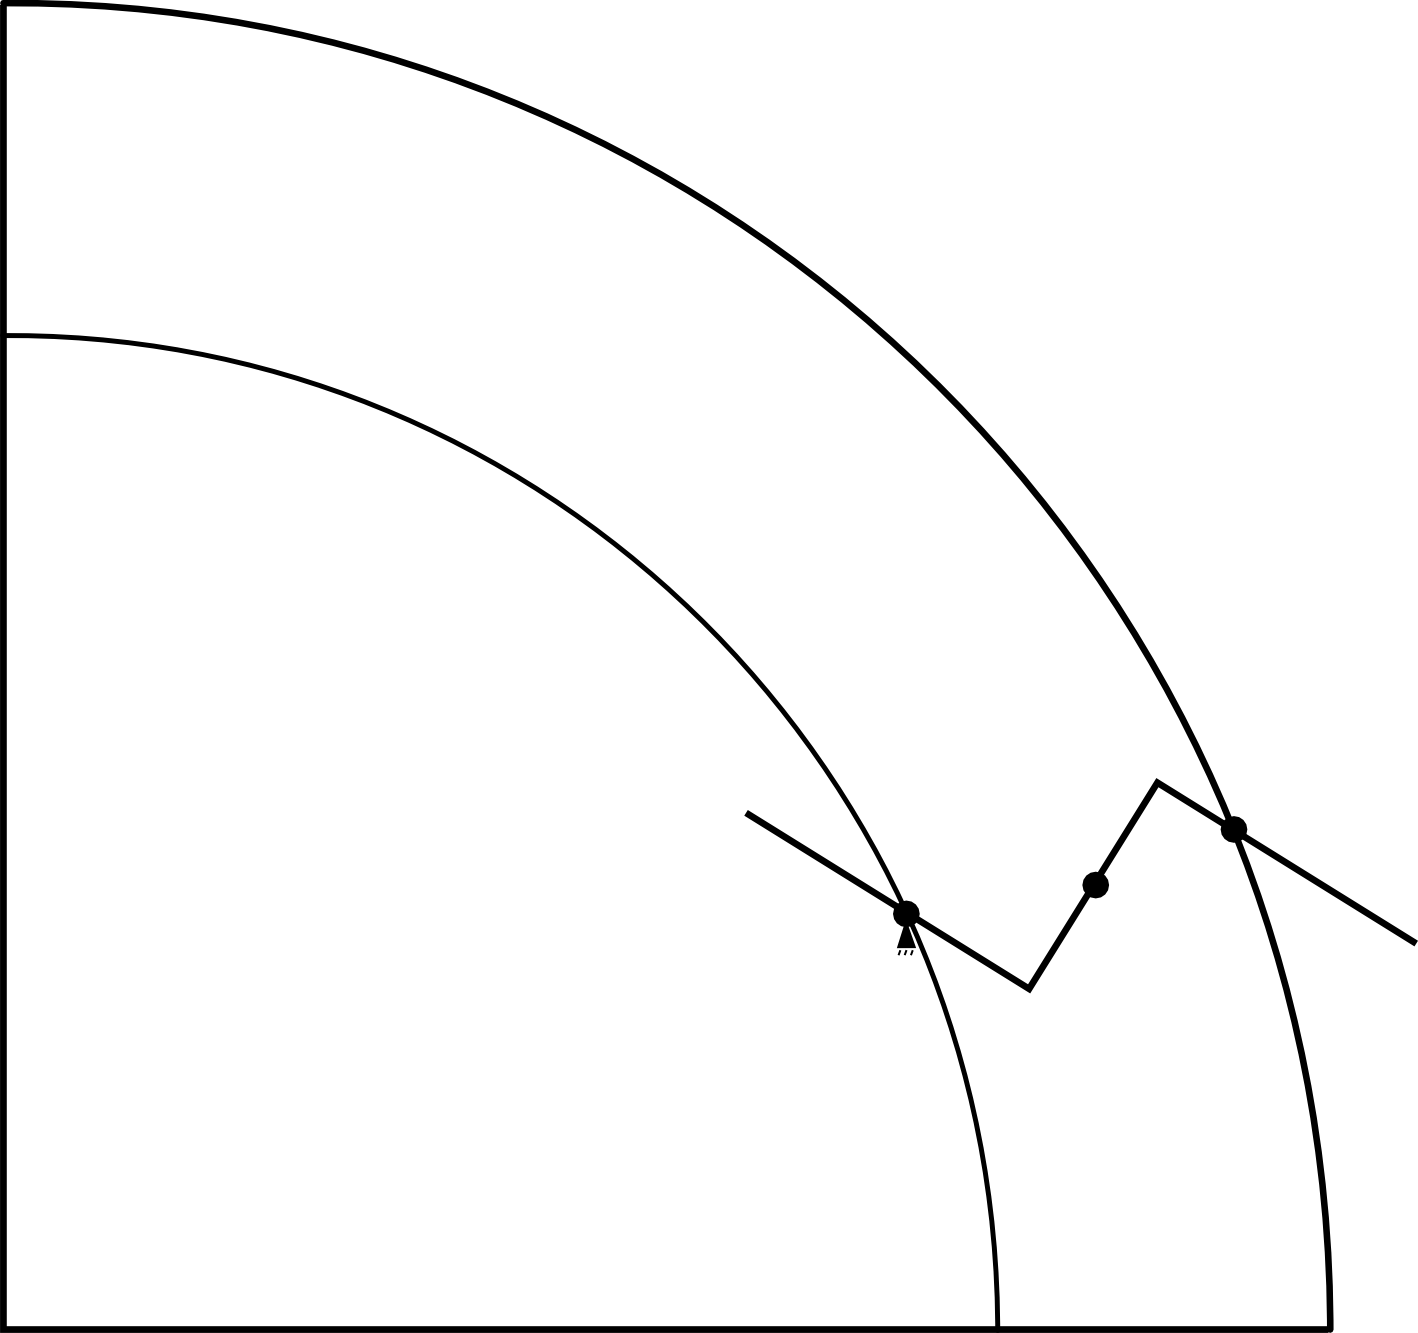
\includegraphics[width=40mm]{lateral_step1}\\1}
\end{minipage}
\begin{minipage}{0.49\linewidth}
\center{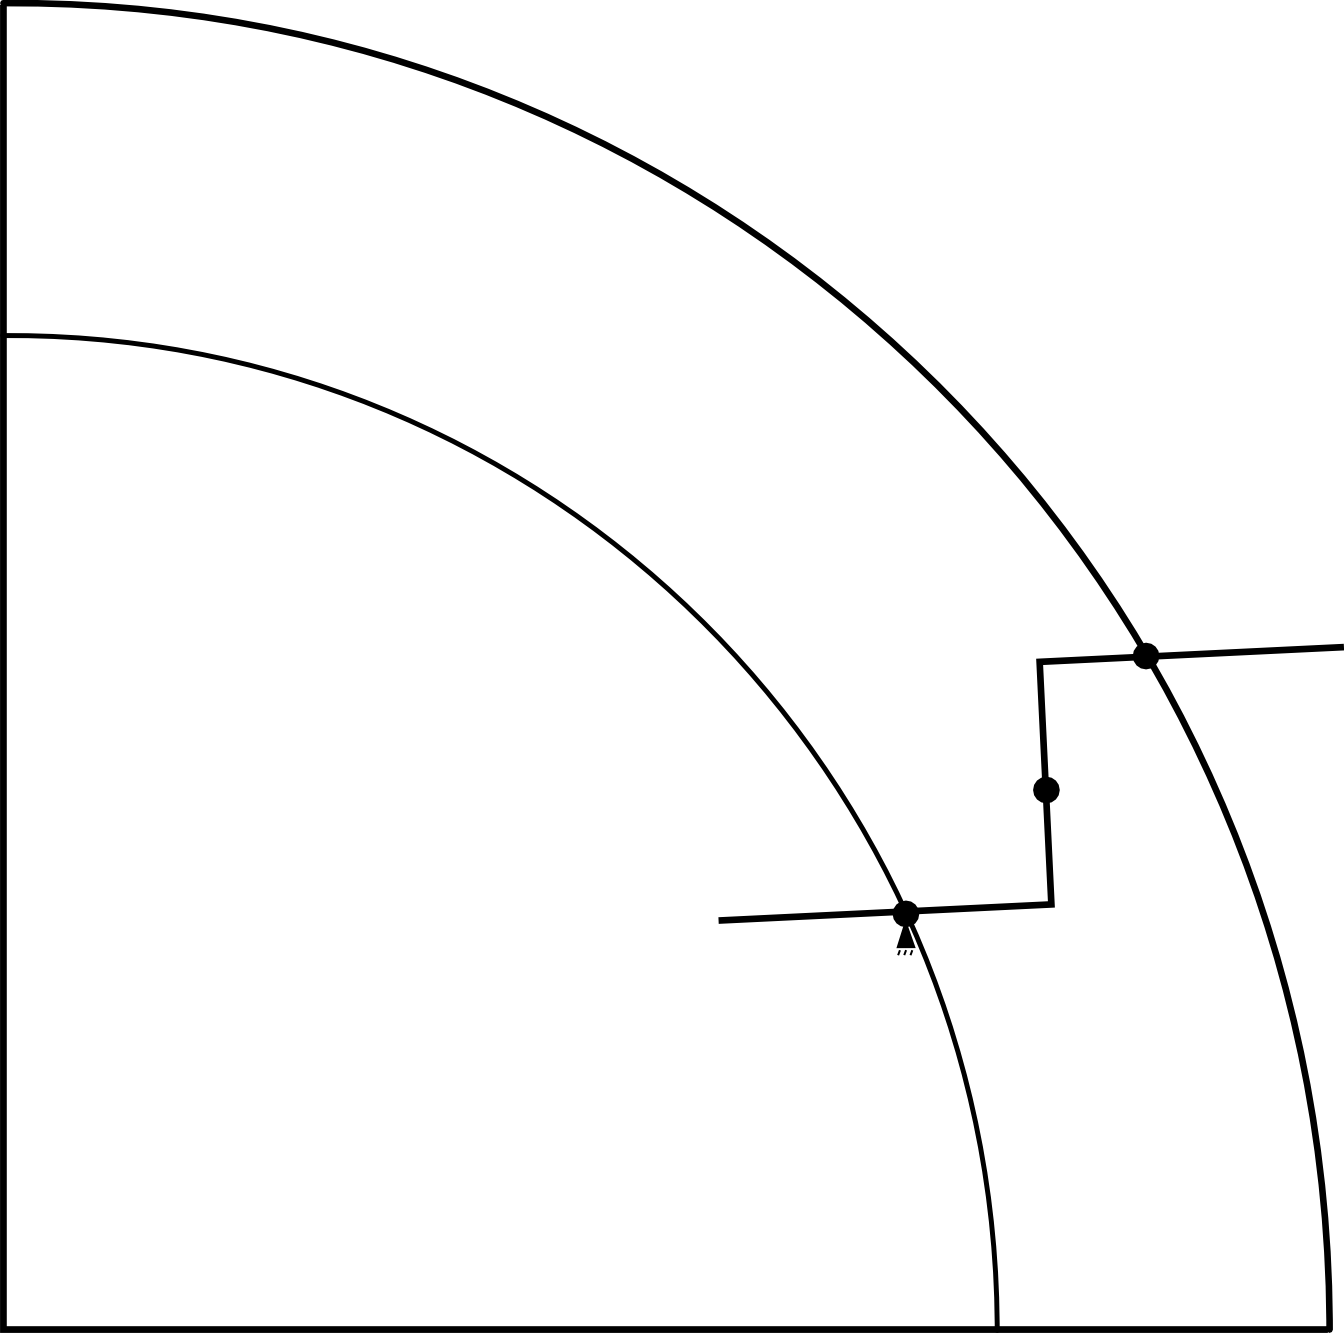
\includegraphics[width=40mm]{lateral_step2}\\2}
\end{minipage}
%\begin{minipage}{0.49\linewidth}
\center{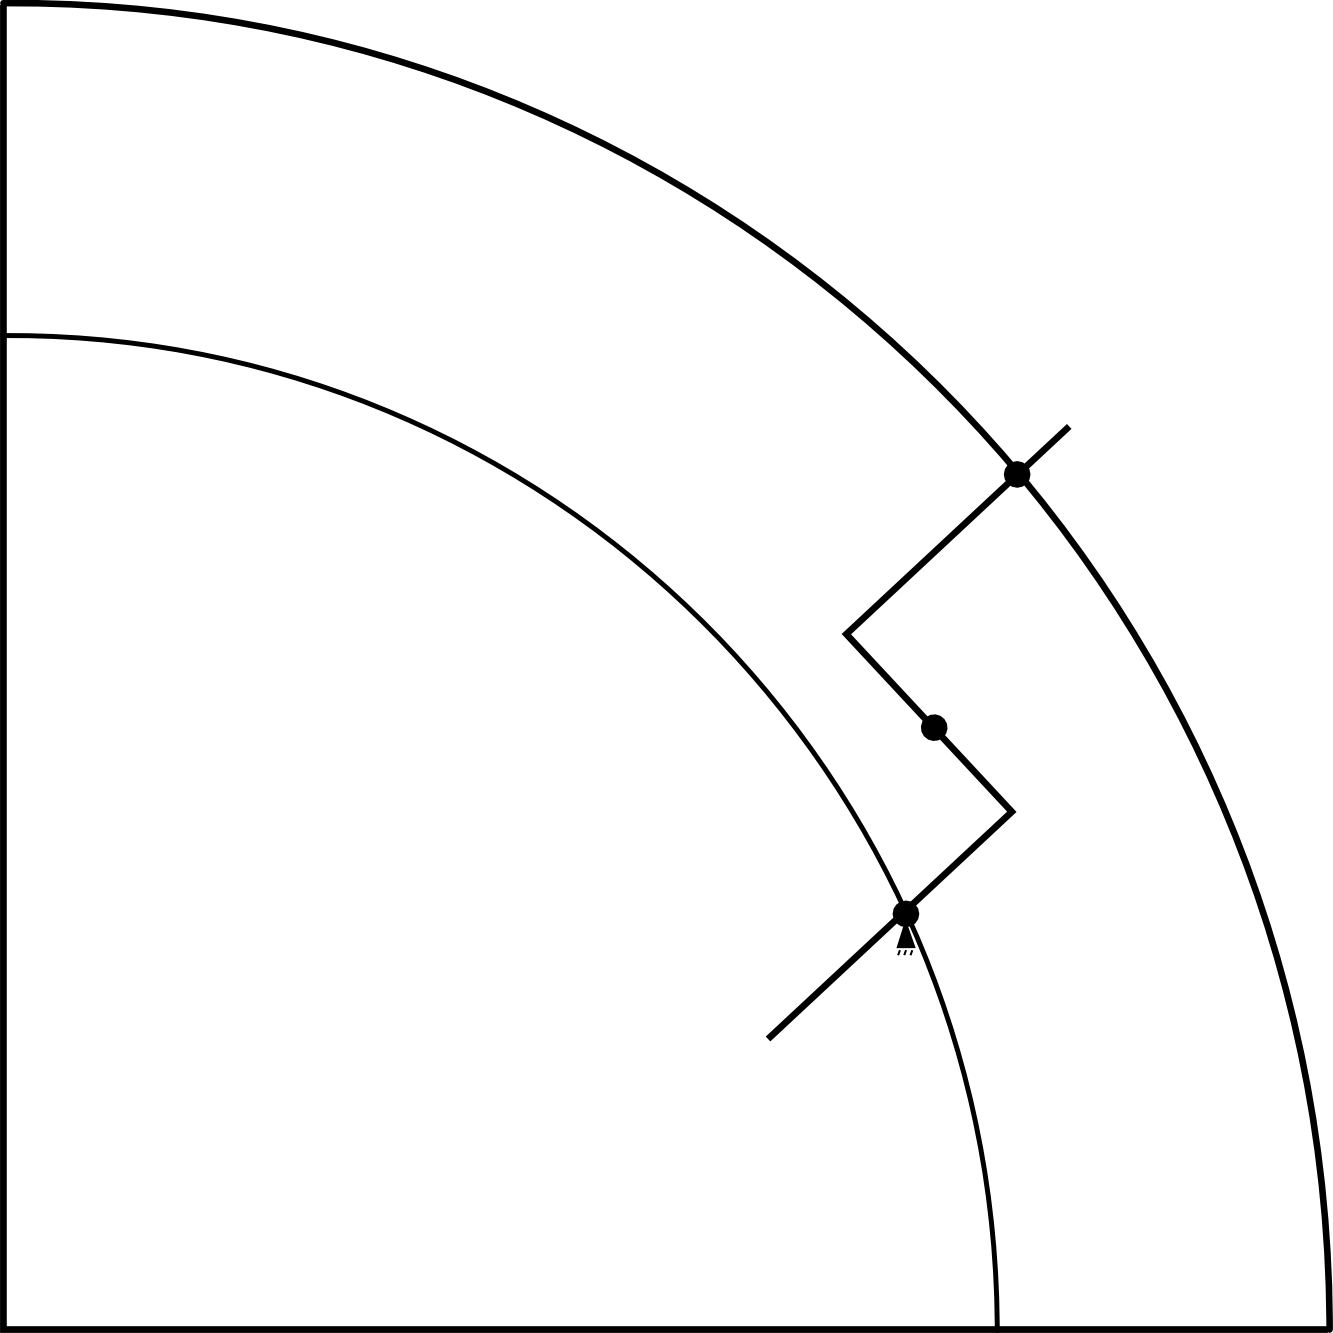
\includegraphics[width=40mm]{lateral_step3}\\3}
%\end{minipage}
\caption{Схема поперечного шага для Н-модуля}
\label{lateral_step}
\end{figure}



%\subsection{Нахождение поступательных степеней свободы Н-модуля}
При движении поперечным шагом знаки координат $d_l$ и $d_r$ постоянны и противоположны. Центр Н-модуля двигается по окружности в положительном направлении, против часовой стрелки. Ноги поочередно ставятся на опорную плоскость, а относительный угол поворота Н-модуля относительно корпуса совершает некоторые колебания около своего нулевого положения.

Будем считать, что все опорные точки для каждой из ног будут выбираться из точек следующих окружностей:

\begin{equation}
	\begin{array}{lcr}
	x^2+(y+R)^2 = (R+r_1)^2\\
	x^2+(y+R)^2 = (R-r_2)^2\\
	\end{array}
	\label{step_circles}
\end{equation}

где $r_1,r_2>0-$ параметры, определяющие радиусы окружностей на которые опираются ноги.

\begin{figure}
\center{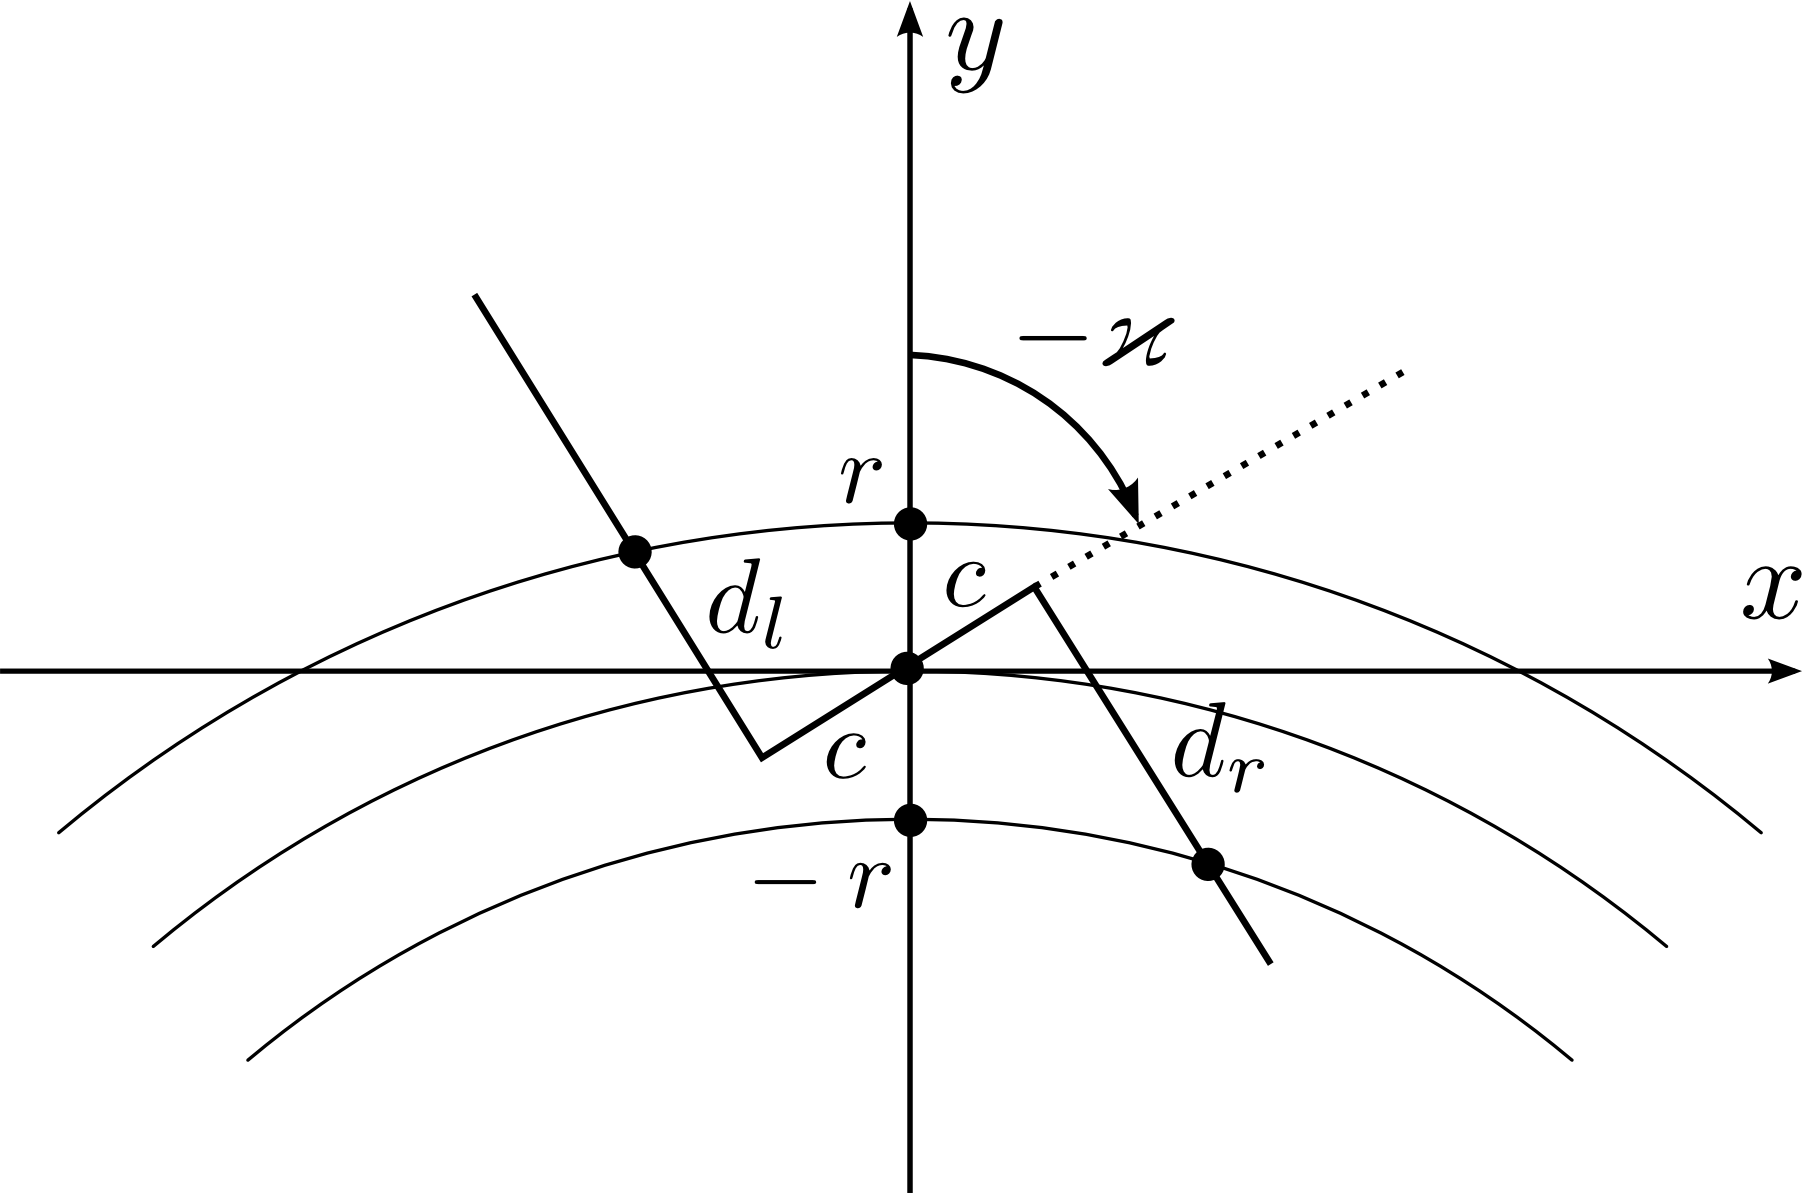
\includegraphics[width=100mm]{ortho_dldr}}
\caption{Задача о нахождении $d_r$ и $d_l$ по углу $\kappa$}
\label{dldrdraw}
\end{figure}

Будем считать, что левая нога модуля будет опираться на точки большей окружности, а правая нога модуля на точки  меньшей окружности. По известному углу $\kappa$ (рис. \ref{dldrdraw}) найдем $d_r$ и $d_l$, используя координатный метод.

Уравнения прямых $l_r$ и $l_l$, проходящих через отрезки поступательных степеней свободы Н-модуля в векторном виде выглядят следующим образом:

\begin{equation}
\begin{array}{c}
l_r:
\left( \begin{array}{c}
x\\
y\\
\end{array}\right) = c \left(\begin{array}{r}
-\sin{\kappa}\\
\cos{\kappa}\\
\end{array}\right)+d_r\,\left(\begin{array}{r}
-\cos{\kappa}\\
-\sin{\kappa}\\
\end{array}\right)\\
\\
l_l:
\left( \begin{array}{c}
x\\
y\\
\end{array}\right) = c \left(\begin{array}{r}
\sin{\kappa}\\
-\cos{\kappa}\\
\end{array}\right)+d_l\,\left(\begin{array}{r}
-\cos{\kappa}\\
-\sin{\kappa}\\
\end{array}\right)\\
\end{array}
\end{equation}

Точки прямых должны удовлетворять соответствующим уравнениям (\ref{step_circles}). После всех преобразований получаем квадратные уравнения относительно $d_r$ и $d_l$:

\begin{equation}
\left\{
\begin{array}{lcr}
d_r^2-2Rd_r\sin{\kappa}+c^2+2Rc\cos{\kappa}+2Rr_1-r_1^2=0\\
\\
d_l^2-2Rd_l\sin{\kappa}+c^2-2Rc\cos{\kappa}-2Rr_2-r_2^2=0\\
\end{array}
\right.
\label{drdl}
\end{equation}

Решения системы (\ref{drdl}) имеют вид:

\begin{equation}
\left\{
\begin{array}{lcr}
d_r = R\sin{\kappa}\pm(R^2\sin^2{\kappa}-2Rc\cos{\kappa}-2Rr_1+r_1^2-c^2)^{\frac{1}{2}}\\
\\
d_l = R\sin{\kappa}\pm(R^2\sin^2{\kappa}+2Rc\cos{\kappa}+2Rr_2+r_2^2-c^2)^{\frac{1}{2}}\\
\end{array}
\right.
\label{dldrsolutions}
\end{equation}

Два решения для каждой степени свободы $d_r, d_l$ следуют из того, что прямая на плоскости пересекает окружность либо в двух различных точках, либо в одной точке, либо не пересекает окружность  вообще. Количество решений и их выбор зависит от значения угла $\kappa$. Угол $\kappa$ выбран так, что для случая на рисунке (\ref{dldrdraw}) подходят решения:

\begin{equation}
\left\{
\begin{array}{lcr}
d_r = R\sin{\kappa}+(R^2\sin^2{\kappa}-2Rc\cos{\kappa}-2Rr_1+r_1^2-c^2)^{\frac{1}{2}}\\
\\
d_l = R\sin{\kappa}+(R^2\sin^2{\kappa}+2Rc\cos{\kappa}+2Rr_2+r_2^2-c^2)^{\frac{1}{2}}\\
\end{array}
\right.
\label{dldrsolution}
\end{equation}

%\subsection{Область существования решения для поступательных степеней свободы $d_l, d_r$}
Исследуем область существования решений (\ref{dldrsolutions}) в зависимости от безразмерных параметров, определяющих геометрию H-модуля: 

$$
\xi = \dfrac{c}{R}, \eta = \dfrac{r}{R}
$$

Рассмотрим области существования решений для $d_r$ и $d_l$. Условие существования решения для $d_r$ равносильно условию неотрицателности соответствующего подкоренного выражения из (\ref{dldrsolution}):

\begin{equation}
R^2\sin^2{\kappa}-2Rc\cos{\kappa} -2Rr+r^2-c^2\geq0\\
\end{equation}

В безразмерных координатах это условие записывается в виде:

\begin{equation}
\eta^2-2\eta+(\sin^2{\kappa}-2\xi\cos{\kappa}-\xi^2)\geq0\\
\label{etaxi}
\end{equation}

Построим решение полученного неравенства на плоскости $(\xi,\eta)$. Построим границы области решения $\eta = \eta(\xi)$:

\begin{equation}
\eta_{1,2} = 1\pm(\cos{\kappa}+\xi)
\label{xietasolution}
\end{equation}

Области решения неравенства (\ref{etaxi}) для правой ноги на плоскости выглядят следующим образом:

\begin{figure}[!h]
\center{\includegraphics[width=100mm]{pic4_1}}
\caption{Область решения неравенства (\ref{etaxi})}
\end{figure}

Область решений неравенства (\ref{etaxi}) зависит от значения угла $\kappa$. При повороте Н-модуля, угол $\kappa$ будет последовательно проходить значения из интервала $[0,2\pi]$. При этом, область из решения (\ref{etaxi}) будет смещаться на плоскости $(\xi,\eta)$. Физический смысл параметров $(\xi,\eta)$ состоит в том, что каждая точка на плоскости $(\xi,\eta)$ это определенная конструкция Н-модуля и фиксированная следовая колея. Если при прохождении угла $\kappa$ своего рабочего диапазона область решения покрывает точку соответствующую данной конструкции Н-модуля, то значит мы можем поставить ногу на соответствующую опорную окружность. Построения на плоскости $(\xi,\eta)$ пригодятся на этапе выбора ширины Н-модуля и определения ширины следовой колеи для ног.

Аналогично получаем для радикала из выражения (\ref{dldrsolution}) для $d_l$:

\begin{equation}
\eta^2+2\eta+(\sin^2{\kappa}+2\xi\cos{\kappa}-\xi^2)\geq0
\end{equation}

\begin{equation}
\eta_{1,2} = -1\pm(\cos{\kappa}-\xi)
\end{equation}

Область существования решений для пересечения левой ноги с большей окружностью:

\begin{figure}[!h]
\center{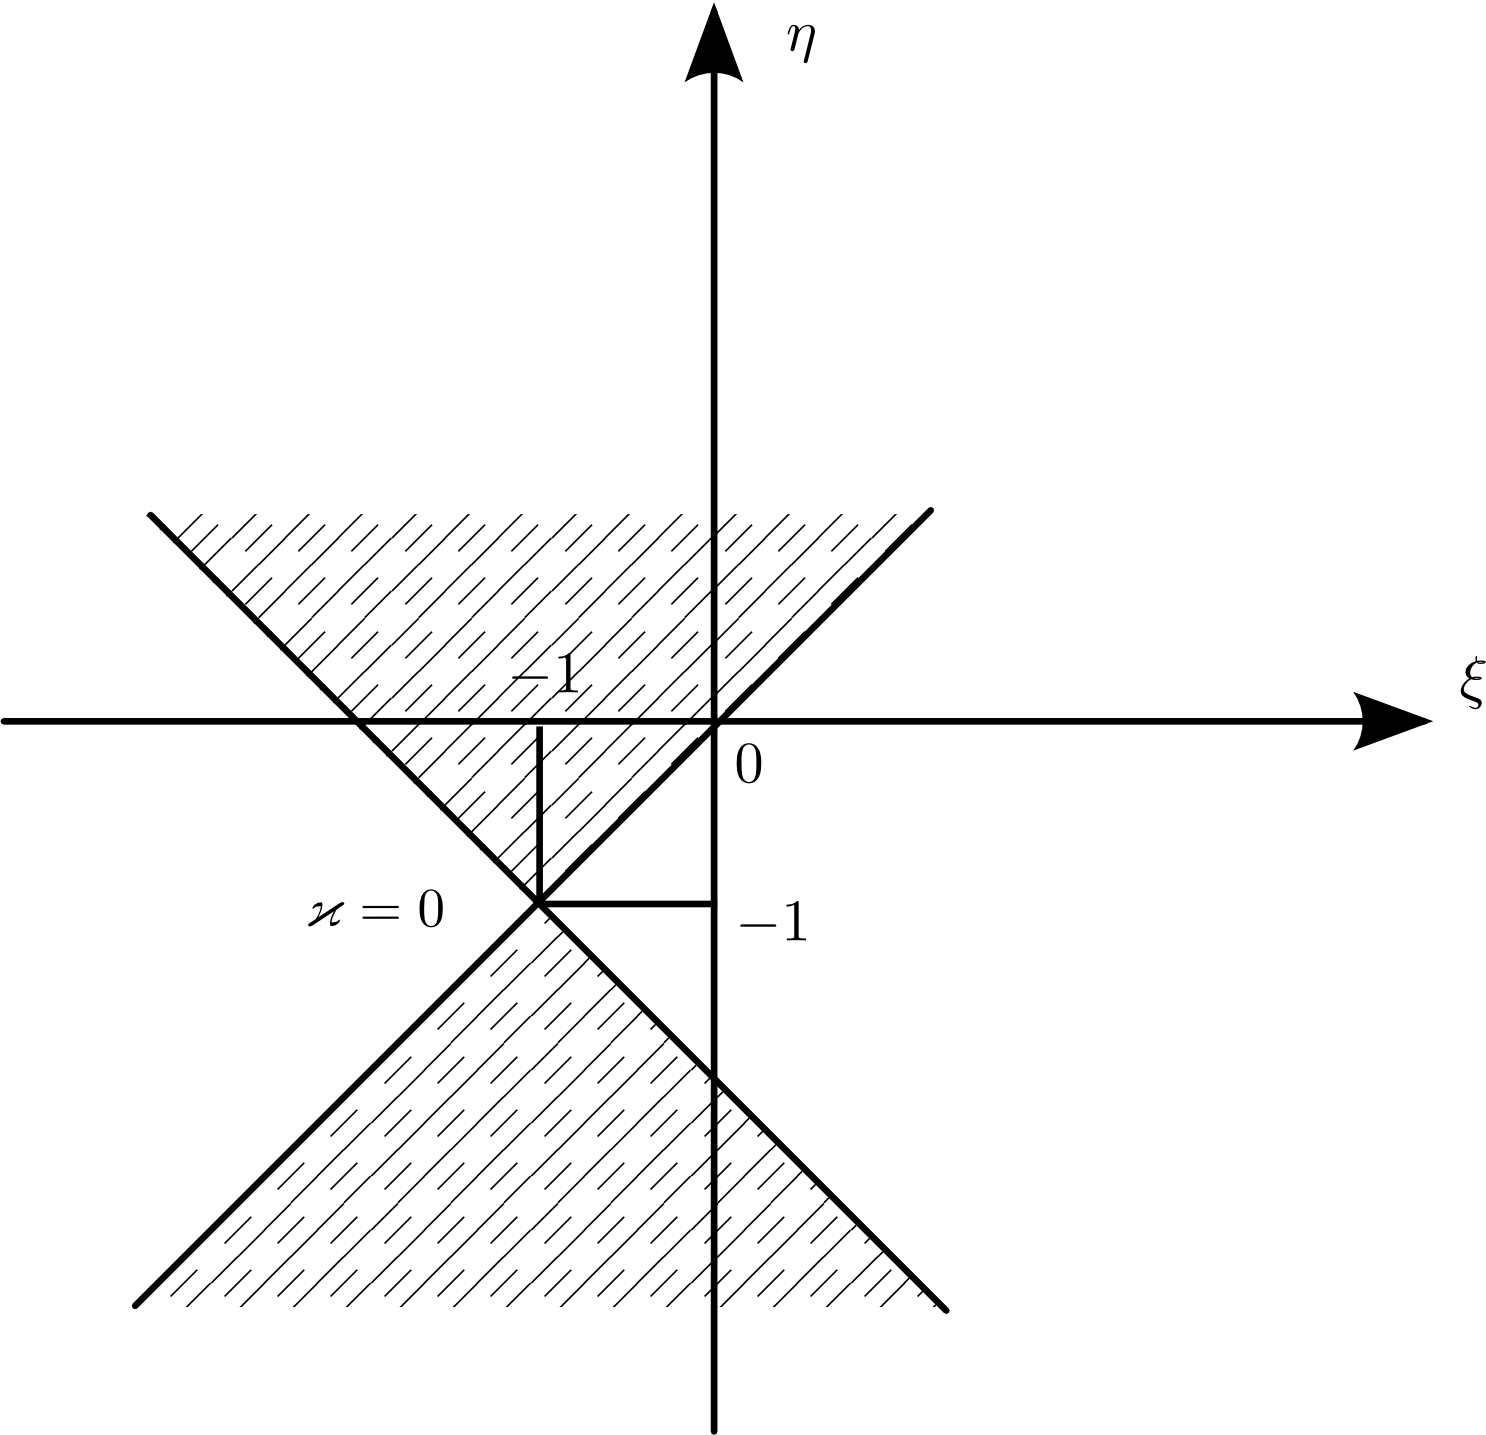
\includegraphics[width=80mm]{pic4_1left}}
\caption{Область существования решений для левой ноги}
\end{figure}

Приведенные решения неравенств для подкоренных выражений из формул для $d_l,d_r$ не подразумевает какого-либо ограничения на модуль $d_l,d_r$. В реальном аппарате максимальная длина поступательных степеней свободы $|d_i|$ будет ограничена некоторой постоянной величиной $d_{max}$. Ограничение на модуль поступательных степеней будет влиять на форму области существования решения в безразмерном пространстве параметров.

%\subsection{Область существования решений с учетом ограничения на поступательные степени $|d_l|,|d_r|\leq d_{max}$}
Исследуем влияние ограничения $|d_r|\leq d_{max}= C = const$ на область существования решений (\ref{dldrsolutions}). Расширим пространство $(\xi,\eta)$, добавим еще одну безразмерную координату $\rho = \dfrac{d_{max}}{R}$. Условие ограниченности решения для $d_r$ примет вид:

\begin{equation}
\left|R\sin{\kappa}+\left(R^2\sin^2{\kappa}-2Rc\cos{\kappa}-2Rr+r^2-c^2\right)^{\frac{1}{2}}\right|\leq d_{max}
\label{ineq1}
\end{equation}

Пусть угол $\kappa$ положителен и достаточно мал. Тогда, выражение под знаком модуля раскрывается со знаком плюс и в безразмерных координатах неравенство (\ref{ineq1}) запишется в виде:

\begin{equation}
\eta^2-2\eta-2\xi\cos{\kappa}-\xi^2-\rho^2+2\rho\sin{\kappa}\leq 0\\
\label{ineq2}
\end{equation}

Используя основное тригонометрическое тождество можно выделить полные квадраты. После преобразования неравенство (\ref{ineq2}) принимает вид:

\begin{equation}
(\eta-1)^2-(\xi+\cos{\kappa})^2-(\rho-\sin{\kappa})^2 \leq 0\\
\label{cone}
\end{equation}

В пространстве $(\xi,\eta,\rho)$ уравнение $(\eta-1)^2-(\xi+\cos{\kappa})^2-(\rho-\sin{\kappa})^2 = 0$ задает поверхность второго порядка - круговой конус. Ось симметрии конуса направлена вдоль оси $O\eta$. Область решения неравенства представлена на рисунке (\ref{3dineq}). Область допустимых значений не зависит от значения параметра $\rho$ и соответствует части пространства заключенного между пересекающимися плоскостями из (\ref{xietasolution}). Неравенство (\ref{cone}) отсекает из области допустимых значений точки, лежащие строго внутри конуса. Область решений зависит от значения угла $\kappa$. При изменении угла $\kappa$ в интервале $[0,2\pi]$ центр конуса двигается по окружности единичного радиуса: $(-cos(\kappa),\eta=1,sin(\kappa))$. Область допустимых значений так же будет смещаться вслед за конусом.

\begin{figure}
\center{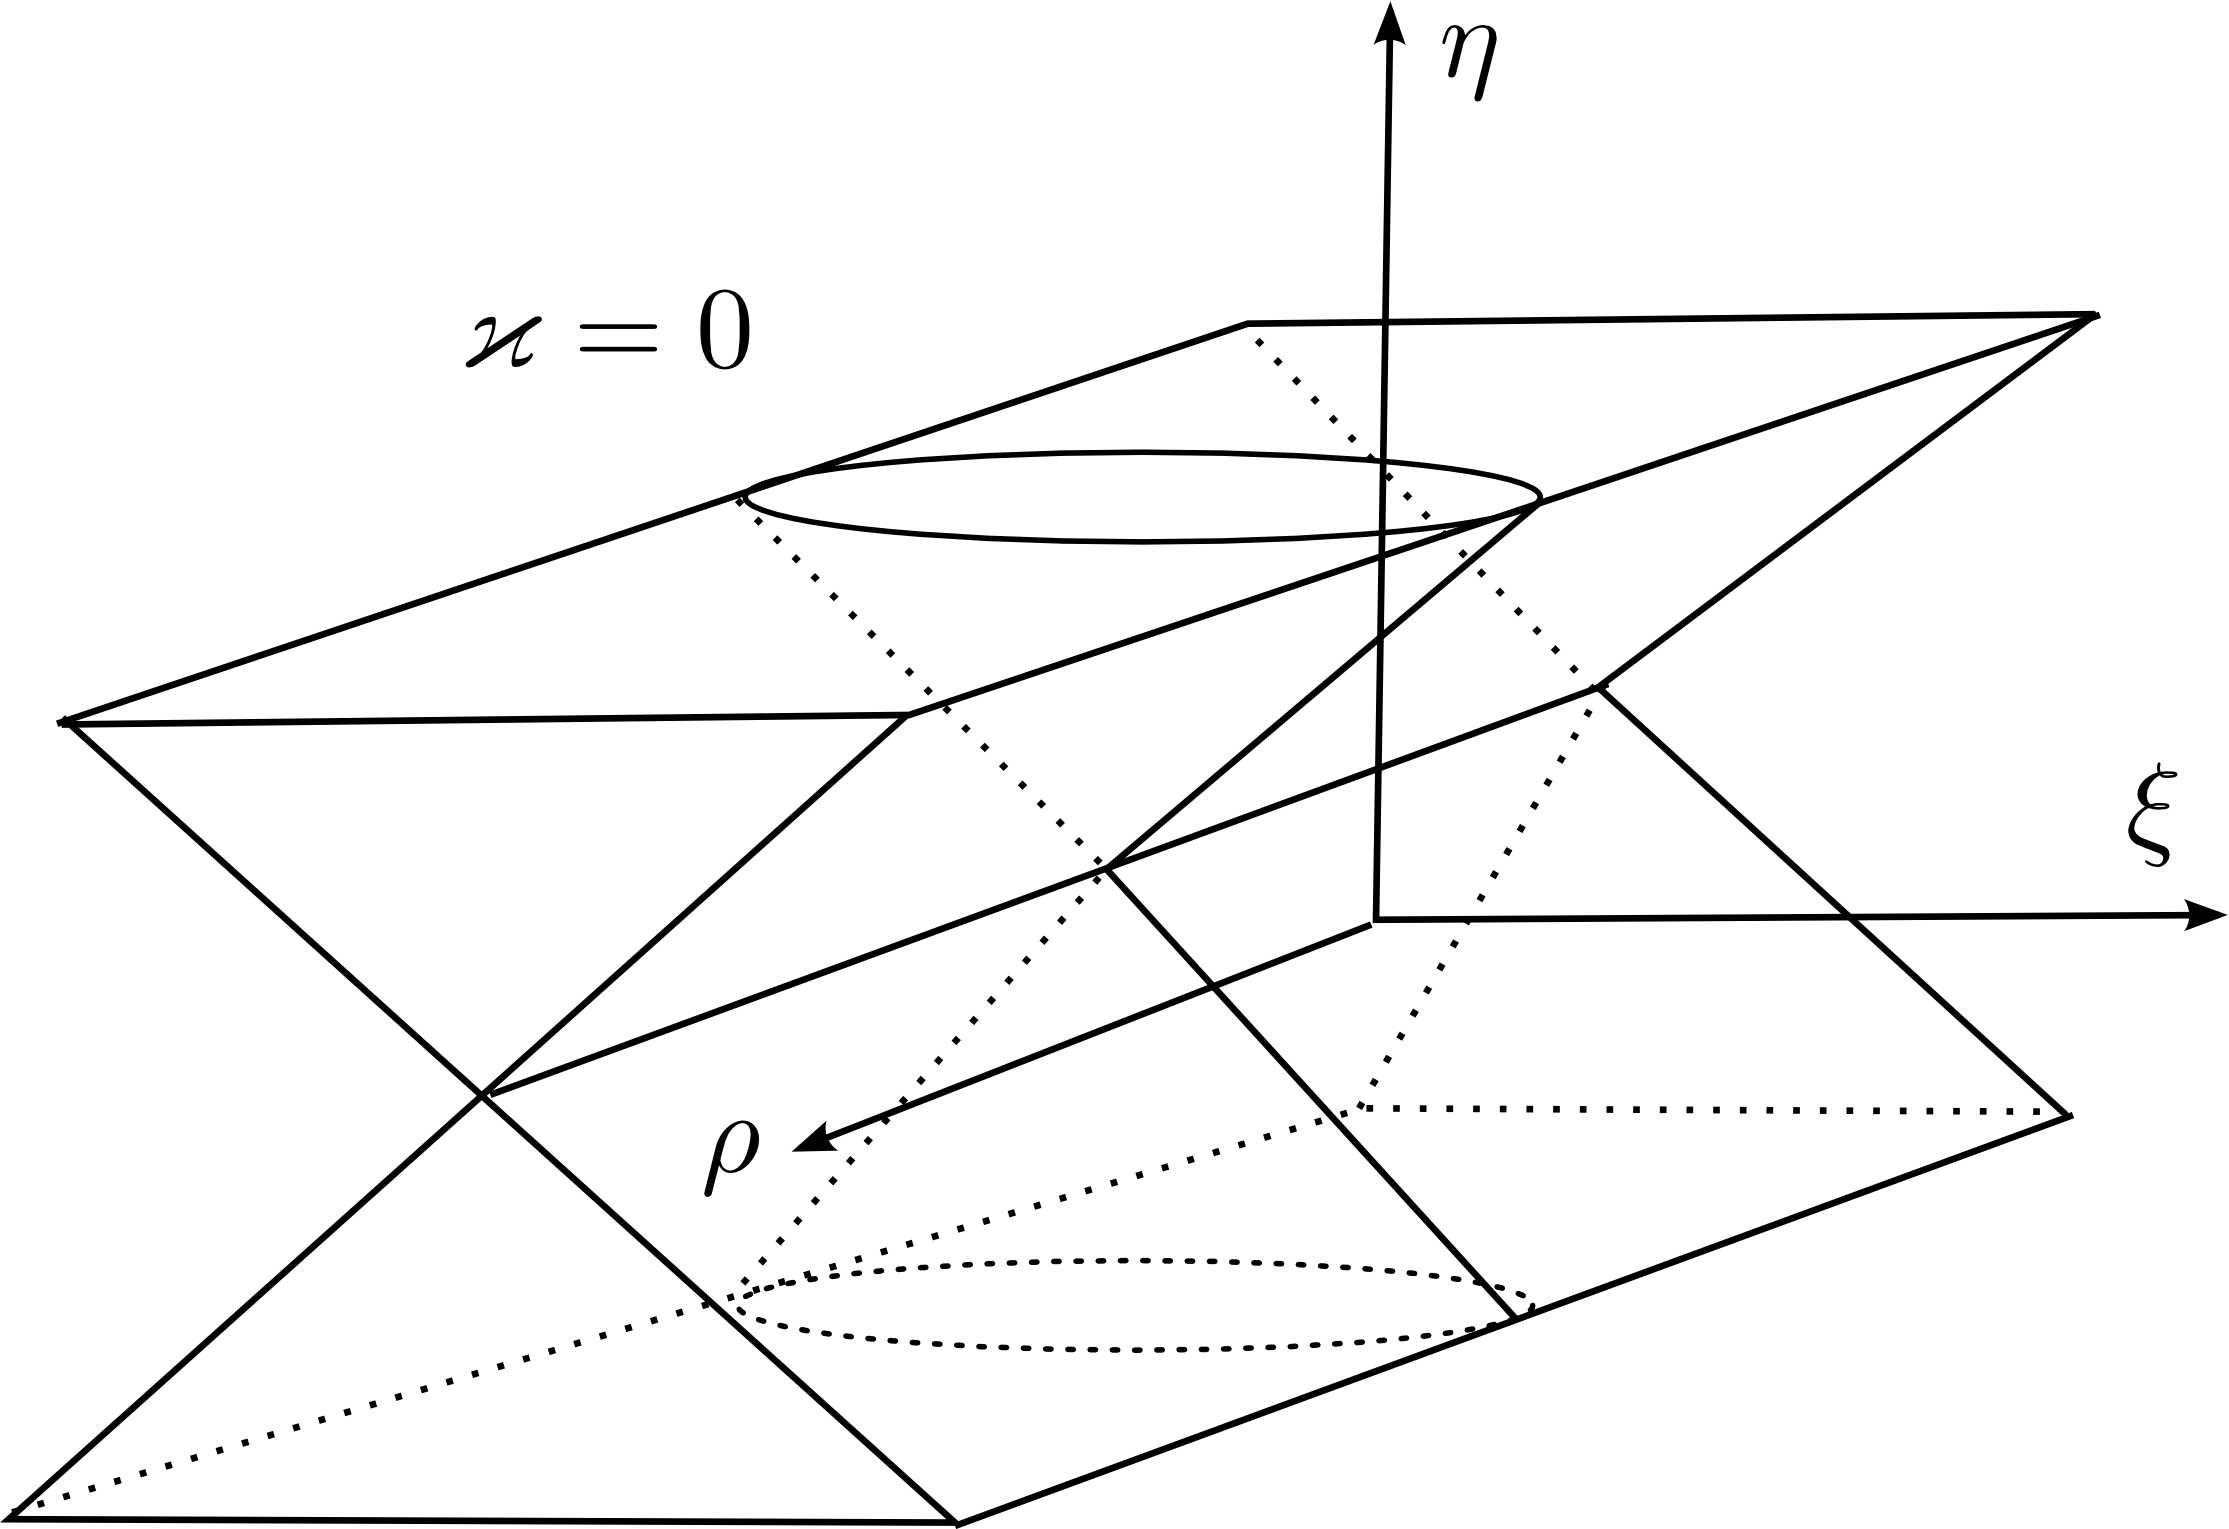
\includegraphics[width=100mm]{3dparam}}
\caption{Трехмерная область решения неравенства (\ref{ineq2})}
\label{3dineq}
\end{figure}

При каждом фиксированном значении параметра $\rho$ будет происходить сечение кругового конуса плоскостью $\rho=const$. В результате сечения будут образовываться кривые второго порядка - гиберболы:

\begin{equation}
(\eta-1)^2-(\xi+\cos{\kappa})^2 = (d_{max}-\sin{\kappa})^2
\end{equation}

 При каждом фиксированном $\kappa$ область существования решений будет зажата между пересекающимися прямыми и ветвями гиперболы:

\begin{figure}
\center{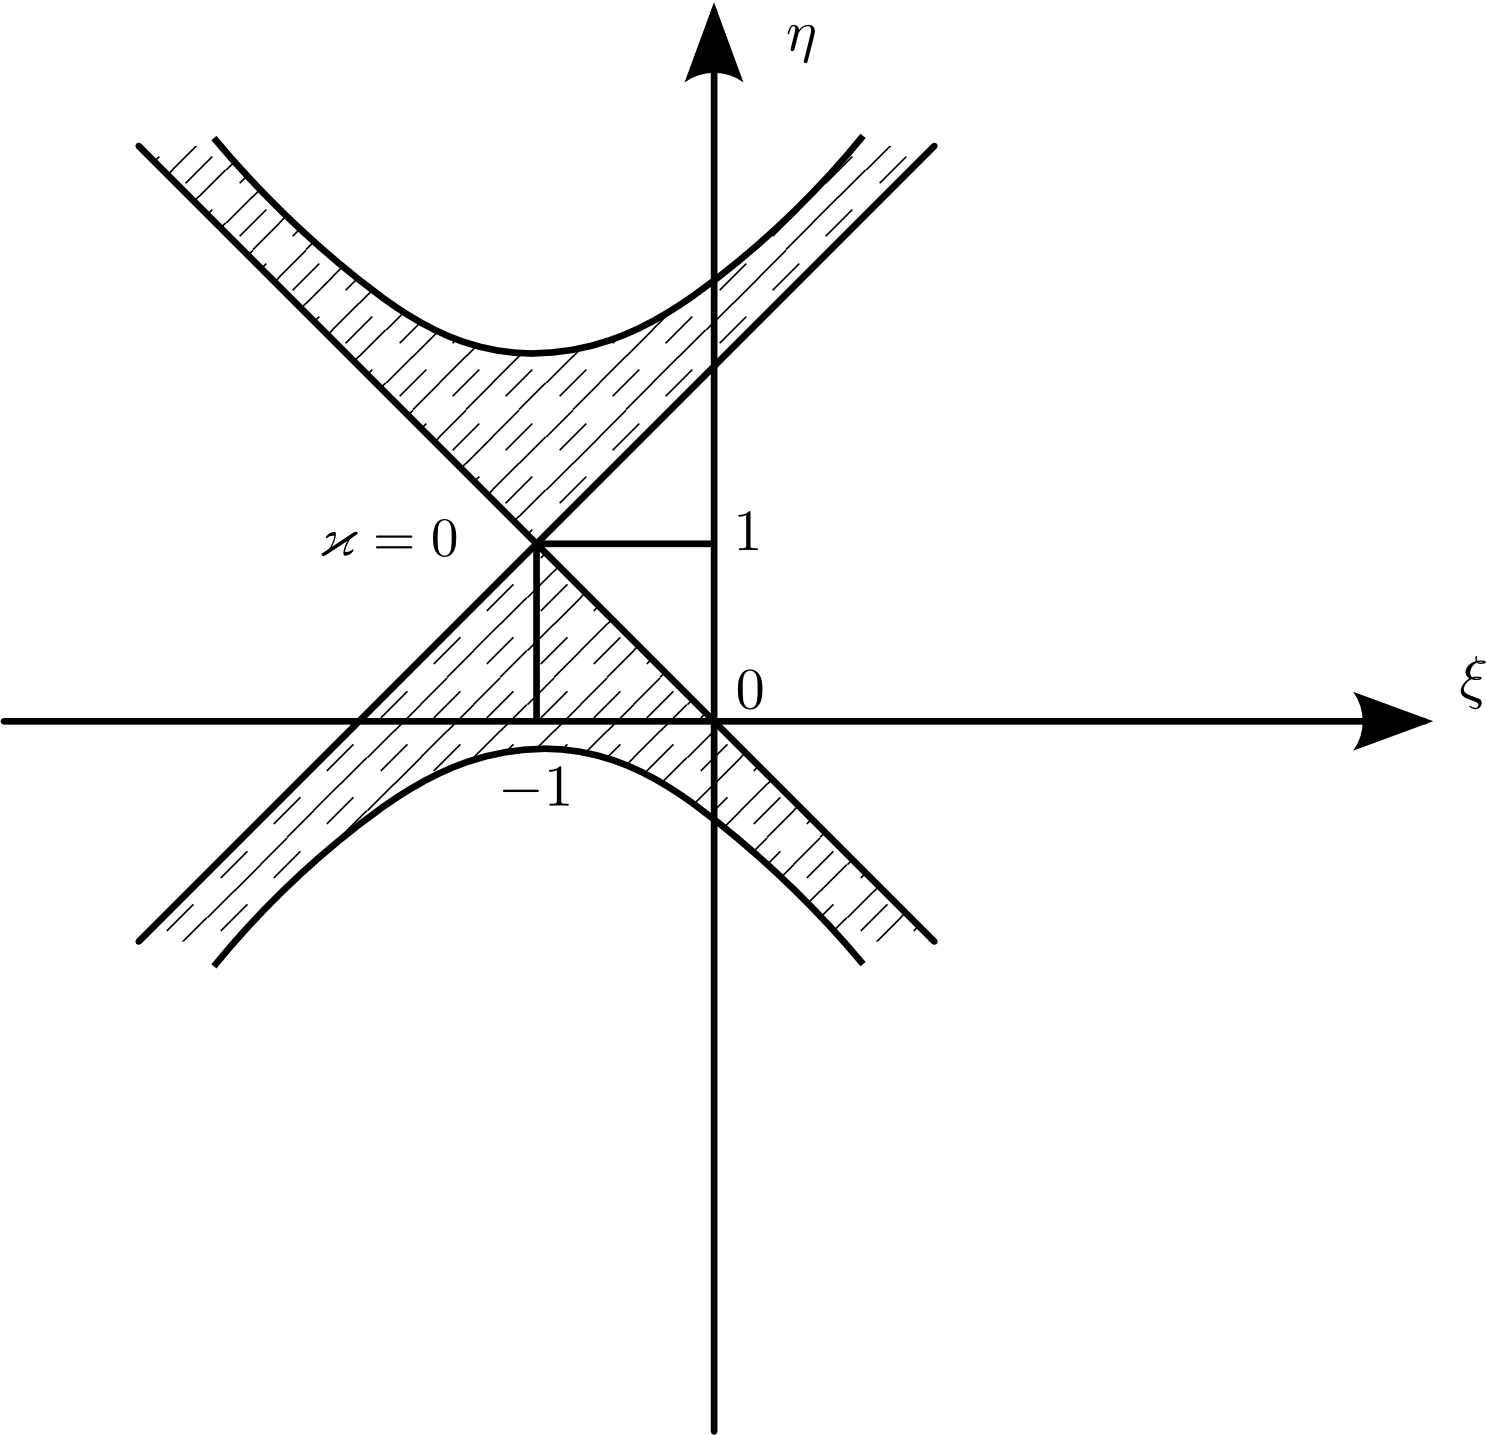
\includegraphics[width=100mm]{pic5}}
\caption{Сечение плоскостью $\rho=d_{max} = const$}
\end{figure}

Аналогичные выкладки для пространства безразмерных параметров проводятся для левой ноги Н-модуля.

Каждая точка пространства $(\xi,\eta,\rho)$ определяет фиксированное соотношение между конструкционными параметрами $c, R = \sqrt{a^2+b^2}$ и $d_{max}$; параметр $r$ отвечает за выбор следовых точек и является независимой переменной. Практический интерес представляет область $M = \{(\xi,\eta,\rho):\xi \in [0,1], \eta \in [0,1], \rho \in[0,1]\}$. Точки лежащие вне области $M$ соответствуют неправдоподобным соотношениям геометрических размеров Н-модулей, размерам корпуса аппарата и расположением следовых точек. Так, например, точка $(\xi,\eta,\rho) = (1,1,1)$ соответствует соотношению $c = R, r = R, d_{max} = R$. При таком соотношении, меньшая опорная окружность становится окружностью нулевого радиуса и схлопывается в точку, ширина Н-модуля $2\,c = 2\,R$, максимальное значение модуля поступательной степени равно $R$. 

\begin{figure}
\center{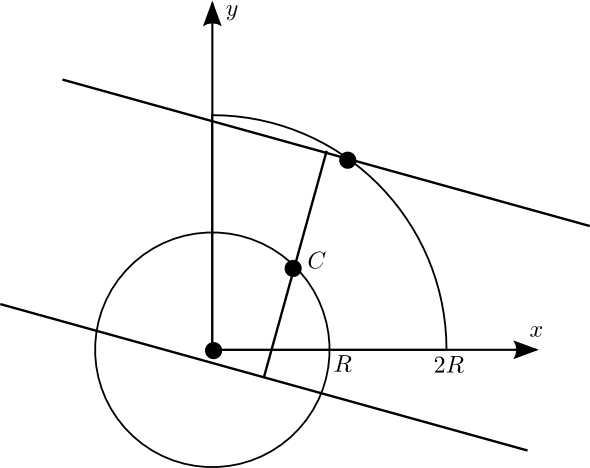
\includegraphics[width=100mm]{pic6}}
\caption{Случай $(\xi,\eta,\rho) = (1,1,1)$}
\end{figure}


Пространство параметров удобно использовать при выборе геометрических параметров шагающего аппарата на этапе проектирования. Зафиксировав точку в пространстве $(\xi,\eta,\rho)$ можно определять амплитуду прокачки угла $\kappa$ и, при необходимости, изменять параметр $\eta$, отвечающий за радиусы опорных окружностей. Проведенное исследование области параметров $(\xi,\eta,\rho)$ относится только к задаче разворота на месте.


\subsection{Максимальный шаг}
Найдем такие $\kappa^l$ и $\kappa^{r}$ при которых координаты $d_l, d_r$ достигают своего максимального значения. Для $d_l$ из (\ref{dldrsolution}) подставляем $d_l=d_{max}$:

$$
d_{max} = R\sin{\kappa^l}+(R^2\sin^2{\kappa^l}+2\,R\,c\cos{\kappa^l}+2\,R\,r+r^2-c^2)^{\frac{1}{2}}\\
$$

$$
d^2_{max}-2\,R\,d_{max}\sin{\kappa^l}+R^2\sin^2{\kappa^l} = R^2\sin^2{\kappa^l}+2\,R\,c\cos{\kappa^l}+2\,R\,r+r^2-c^2\\
$$

После приведения подобных слагаемых перенесем все функции с $\kappa^l$ в одну сторону равенства и разделим обе части на $2\,R$:

$$
c\cos{\kappa^l}+d_{max}\sin{\kappa^l} = \dfrac{d^2_{max}+c^2-r^2-2\,R\,r}{2\,R\\}
$$

Разделим обе части равенства на $\sqrt{c^2+d^2_{max}}$, воспользуемся формулой вспомогательного угла и получим:

$$
\sin{(\psi+\kappa^l)} = \dfrac{d^2_{max}+c^2-r^2-2\,R\,r}{2\,R\sqrt{c^2+d^2_{max}}}
$$

где $\psi = -\arccos{\left(\dfrac{d_{max}}{\sqrt{c^2+d^2_{max}}}\right)}$, тогда:

$$
\kappa^l = arccos\left(\dfrac{d_{max}}{\sqrt{c^2+d^2_{max}}}\right)\pm arccos\left(\dfrac{d^2_{max}+c^2-2\,r\,R-r^2}{2R\sqrt{c^2+d^2_{max}}}\right)
$$

Аналогично вычисляем $\kappa^{r}$ для $d_r$:

$$
d_{max} = R\sin{\kappa^r} + (R^2\sin^2{\kappa^r}-2\,R\,c\cos{\kappa^r}-2\,R\,r+r^2-c^2)^\frac{1}{2}
$$

$$
\kappa^r = \arcsin{\left(\dfrac{c}{\sqrt{c^2+d^2_{max}}}\right)}\pm\arcsin{\left(\dfrac{-d^2_{max}-c^2-2\,R\,r+r^2}{2\,R\sqrt{c^2+d^2_{max}}}\right)}
$$

После сравнения полученных величин $\kappa^l$ и $\kappa^{r}$ видно, что координата $d_r$ достигает своего экстремума раньше, чем координата $d_l$. Таким образом, получаем, что шаг правой ногой по меньшей окружности получается длиннее чем шаг левой по большей окружности при повороте корпуса аппарата против часовой стрелки.

Рассмотрим случай когда $d_r=d_l=d_{max}$. Будем изменять радиус большей окружности $R+r$ так, чтобы $d_l$ достигало максимума одновременно с $d_r$, т.е. уравняем величины $d_l$ и $d_r$ через изменение радиуса большей опорной окружности. Из выражения для $d_l$ получим уравнение относительно $r$:

\begin{equation}
r^2+2Rr-(d^2_{max}-2d_{max}R\sin\kappa^*-2Rc\cos{\kappa^*}+c^2)=0\\
\end{equation}

Откуда получим:
\begin{equation}
r = -R+(R^2+d^2_{max}-2d_{max}R\sin{\kappa^*}-2Rc\cos{\kappa^*}-c^2)^\frac{1}{2}
\end{equation}

Новый радиус большей опорной окружности:
\begin{equation}
R:=(R^2+d^2_{max}-2d_{max}R\sin{\kappa^*}-2Rc\cos{\kappa^*}-c^2)^\frac{1}{2}
\end{equation}

Далее в работе для простоты будем считать $r_1 = r_2 = r$, т.е. максимальные линейные величины шагов $d_l$ и $d_r$ будут различны.

%\subsection{Угловые величины шага}

Определим углы $\lambda_l$ и $\lambda_r$ как показано на рисунке \ref{angular_step}. Точка $O$ - общий центр опорных окружностей. Назовем величины $\lambda_l$ и $\lambda_r$ угловыми величинами левого и правого шага соответственно.

\begin{figure}
\center{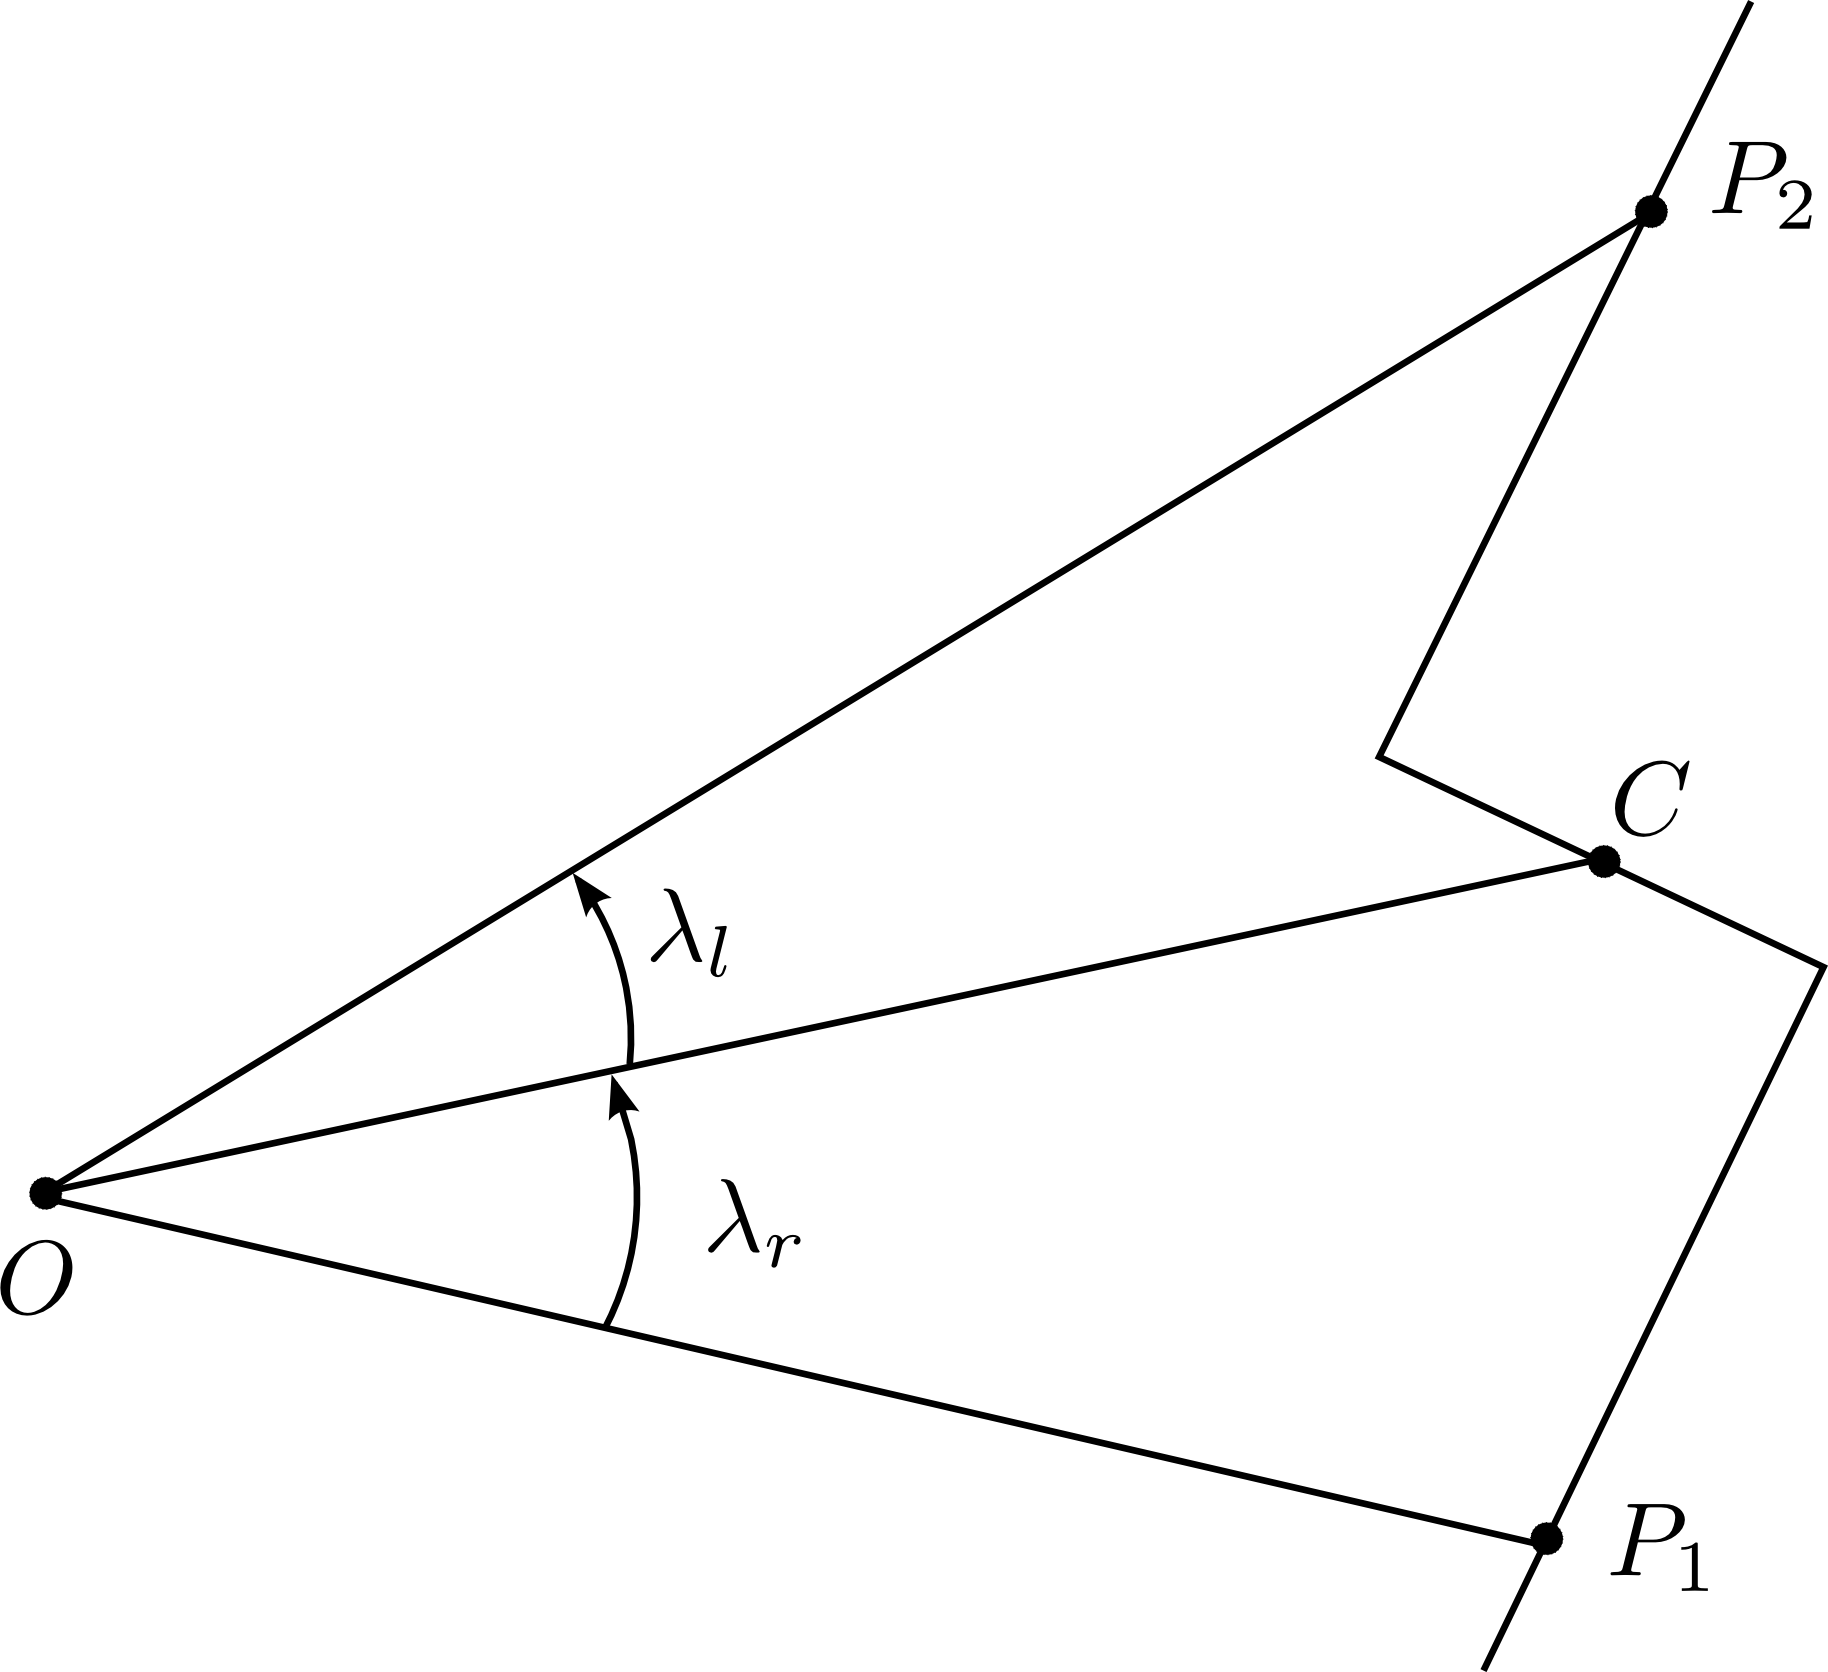
\includegraphics[width=80mm]{ortholambda}}
\caption{Угловые величины шага}
\label{angular_step}
\end{figure}

Используя теорему косинусов находим выражение для $\lambda_l$ и $\lambda_r$:

\begin{equation}
\begin{array}{lcr}
\lambda_r = arccos\left(\dfrac{c^2+d^2_r-R^2-(R-r_1)^2}{2R(R-r_1)}\right)\\
\\
\lambda_l = arccos\left(\dfrac{c^2+d^2_l-R^2-(R+r_2)^2}{2R(R+r_2)}\right)\\
\end{array}
\label{lambdas}
\end{equation}

Найдем координаты опорной точки $P_0$ для правой ноги в начальный момент времени. Координаты точки $P_0 = (a-\sqrt{(R-r_1)^2-(b-c)^2},b-c)$. Для любого другого начального положения Н-модуля можно найти координаты опорной ноги координатным методом.

Рассмотрим движение H-модуля максимальными шагами. Допустим, Н-модуль находится в крайнем возможном по углу $\kappa$ положении, и наступает фаза переноса левой ноги, а правая находится в фазе опоры.

Обозначим $Arg(P_i) := arctan\left(\dfrac{P_{iy}}{P_{ix}}\right)$. Тогда координаты новой опорной точки $P_i$ для левой ноги выражаются через величину угловых шагов:

\begin{equation}
P_i = (R+r)\left(\begin{array}{c}
\cos{(Arg(P_{i-1})+\lambda_r+\lambda_l)}\\
\sin{(Arg(P_{i-1})+\lambda_r+\lambda_l)}\\
\end{array}\right)
\end{equation}


Координаты центра H-модуля получаются по аналогичной формуле

\begin{equation}
C_{i-1,i} = R\left(\begin{array}{c}
\cos{(Arg(P_{i-1})+\lambda_r)}\\
\sin{(Arg(P_{i-1})+\lambda_r)}\\
\end{array}\right)
\end{equation}

\begin{figure}
\center{\includegraphics[width=100mm]{lambda}}
\caption{Cледовые точки при движении максимальными шагами}
\end{figure}

После переноса левой ноги в крайнее положение по углу $\kappa$ наступает фаза переноса правой ноги. Координаты опорной точки для правой ноги:

\begin{equation}
P_{i+1} = (R-r)\left(\begin{array}{c}
\cos{(Arg(P_{i})+\lambda_r+\lambda_l)}\\
\sin{(Arg(P_{i})+\lambda_r+\lambda_l)}\\
\end{array}\right)
\end{equation}

Координаты центра модуля после переноса правой ноги:

\begin{equation}
C_{i,i+1} = R\left(\begin{array}{c}
\cos{(Arg(P_{i})+\lambda_l)}\\
\sin{(Arg(P_{i})+\lambda_l)}\\
\end{array}\right)
\end{equation}

Все последующие опорные точки при движении с максимальным шагом вычисляются аналогично.



%%%Рассмотрим задачу выбора равных шагов по $d_r,d_l$ или $\lambda_l,\lambda_r$. 
%%%
%%%Рассмотрим задачу равенства угловых шагов $\lambda_r = \lambda_l$ при условии $r_1=r_2=r$. Приравнивая выражения (\ref{lambdas}) получаем, что угловые величины шагов равны, когда для $d_r$ и $d_l$ выполнено следующее равенство:
%%%
%%%\begin{equation}
%%%d^2_l = d^2_r\dfrac{(R+r)}{(R-r)}-2r\dfrac{(r^2-c^2)}{(R-r)}
%%%\label{lambdaeq}
%%%\end{equation}
%%%
%%%Подставляя в уравнение (\ref{lambdaeq}) выражения для $d_l,d_r$ из (\ref{dldrsolution}) получим уравнение относительно $\kappa$:
%%%
%%%\begin{equation}
%%%R\sin{\kappa}\left(\sqrt{l}-\sqrt{r}\right)+2Rc\cos{\kappa}+2r\cos^2{\kappa}-r\sin{\kappa}\left(\sqrt{l}+\sqrt{r}\right)=0
%%%\end{equation}
%%%
%%%Это уравнение трудно решается в аналитическом виде. 


%\subsection{Случаи постановки ног в конечные точки}

Рассмотрим последние два шага Н-модуля на пути в конечные следовые точки. Возможны следующие случаи в окрестности конечных следовых точек:
\begin{figure}[h]
\center{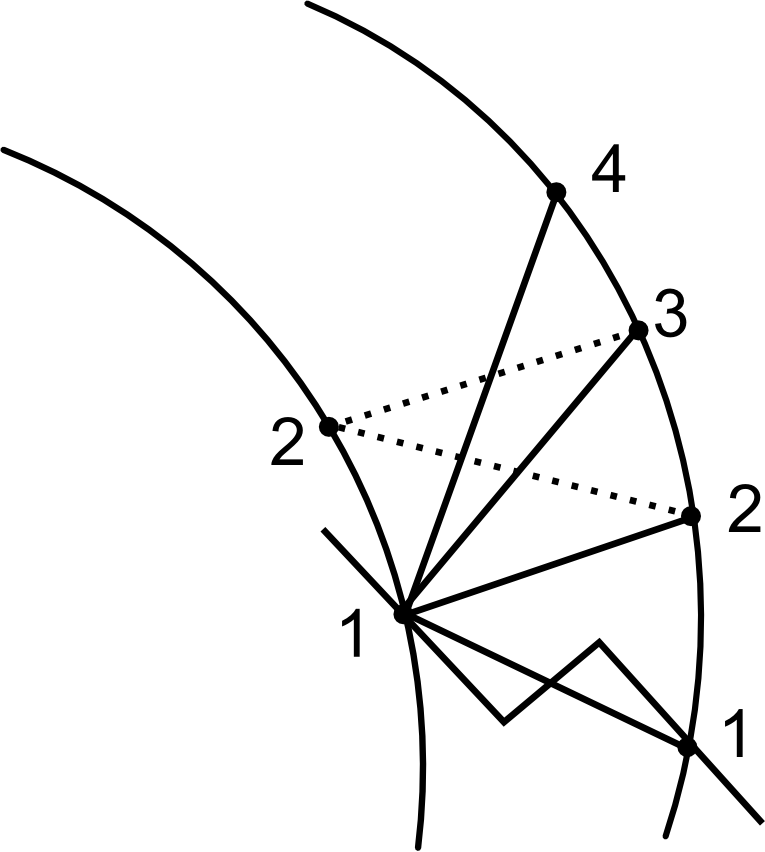
\includegraphics[width=50mm]{orthostepcases}}
\caption{Случаи расположение опорных точек}
\label{stepcase}
\end{figure}

Рассмотрим случаи для шага левой ногой, на рисунке \ref{stepcase}:

Случай (1,1) -  ситуация, когда Н-модуль уже находится в требуемом положении.

Случай (1,2) - правая нога уже находится в требуемом положении, требуется перенести левую ногу в положение номер 2.

Случай (1,3) - положение номер 3 соответствует крайнему положению левой ноги по углу $\kappa$. 

Случай (1,4) - невозможен

Случай (2,1) - невозможен

Случай (2,2) - выполняется в два шага. Сначала переносится левая нога в положение номер 2, и выполняется перенос правой ноги в положение номер 2.

Случай (2,3) - выполняется аналогично случаю (2,2), только при переносе левой ноги угол $\kappa$ уходит в свое максимально возможное положительное значение.

Аналогично рассматриваются случаи для правого шага.

По следовым точкам восстановим значение угла $\kappa$, это позволит синтезировать программное значение угла $\kappa$ для случаев (1,2), (2,2) и (2,3). Заметим, что взаимное положение следовых точек определяется углом между соответствующими радиус векторами следовых точек с точностью до поворота вокруг центра корпуса.

%\subsection{Определение угла $\kappa$ ориентации модуля по паре следовых точеке}

Рассмотрим начальное положение, когда все H-модули имеют нулевые относительные углы поворота. Рассчитаем начальную величину угла $\kappa^0$. Из начального условия находим координаты опорных точек или координаты точек пересечения ног с опорными окружностями. Угол $\kappa$ связан с углом ориентации $\phi$ H-модуля относительно корпуса аппарата: $\kappa = \phi+\dfrac{\pi}{2}+\arctan{\left(\dfrac{b}{a}\right)}$.
%Для начального положения $\kappa^0 = -\dfrac{\pi}{2}-\arctan{\left(\dfrac{b}{a}\right)}$

Пусть известны следовые точки $\overline{P}_1$ и $\overline{P}_2$. Без ограничения общности будем считать, что $\overline{P}_1 = (R-r)(1,0)$, а $\overline{P}_2 = (R+r)\,(cos(\alpha),\sin{\alpha})$. Пусть $p$ - расстояние между опорными точками. Повернем систему координат на угол $\delta := \dfrac{\pi}{2}-\left((Arg(\overline{P}_1)-Arg(\overline{P}_2)-\arcsin\left(\dfrac{2\,c}{p}\right)\right)$. Матрица поворота:

$$
C = \left(\begin{array}{ccc}
\cos{\delta} &-\sin{\delta}\\
\sin{\delta} & \cos{\delta}\\
\end{array}\right)
$$

После преобразования, координаты опорных точек примут вид:

$$
\tilde{P}_1 = C\,\overline{P}_1 = \left(\begin{array}{ccc}
P_{1x}\cos{\delta}\\
P_{1x}\sin{\delta}\\
\end{array}\right),
\tilde{P}_2 = C\,\overline{P}_2 = \left(\begin{array}{ccc}
P_{2x}\cos{\delta}-P_{2y}\sin{\delta}\\
P_{2x}\sin{\delta}+P_{2y}\cos{\delta}\\
\end{array}
\right)
$$

В новой системе координат параллельные прямые проходящие через опорные точки становятся параллельны оси $Oy$. Центр Н-модуля лежит на середине общего перпендикуляра между прямыми, следовательно, абцисса $x_c$ центра $C$ Н-модуля равна:

$$
x_c = \left(\tilde{P}_{1x}+\tilde{P}_{2x}\right)\dfrac{1}{2}
$$

Центр Н-модуля лежит на окружности радиуса $R$, воспользуемся этим условием для нахождения ординаты центра Н-модуля:

$$
y_c = \sqrt{R^2-x^2_c}
$$

Координаты центра Н-модуля в новой системе координат:

$$
\tilde{P}_c = \left( \begin{array}{ccc}
\left(\tilde{P}_{1x}+\tilde{P}_{2x}\right)\dfrac{1}{2}\\
\\
\sqrt{R^2-x^2_c}\\
\end{array}\right)
$$

Выполним переход в исходную систему координат:

$$
\overline{P}_c = C^{-1}\,\tilde{P}_c = \left( \begin{array}{ccc}
x_c\cos{\delta}+y_c\sin{\delta}\\
-x_c\sin{\delta}+y_c\cos{\delta}\\
\end{array}\right)
$$

В начальной системе координат можно выразить искомый угол $\kappa^0$:

$$
Arg(\,\overline{P}_c)+(\pi-Arg(\,\overline{P}_2-\overline{P}_1))+\kappa^0 = \pi,
$$
откуда получаем, что:

\begin{equation}
\kappa^0 = Arg(\,\overline{P}_2-\overline{P}_1)-Arg(\,\overline{P}_c)-\arcsin\left(\dfrac{2\,c}{p}\right)
\end{equation}


\begin{figure}
\center{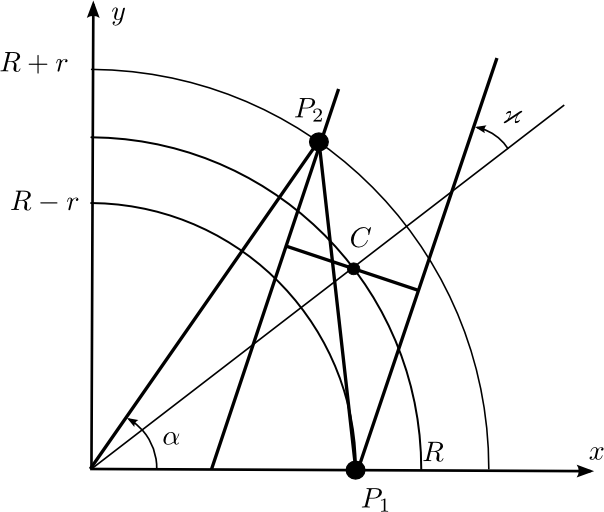
\includegraphics[width=80mm]{ortho_kappa}}
\caption{Нахождение $\kappa^0$ по следовым точкам}
\end{figure}


%\subsection{Синтез управляющего сигнала для $\kappa$ и поступательных степеней $d_l,d_r$}


Теперь есть все необходимые инструменты для нахождения угла $\kappa$ для Н-модуля в различных ситуациях и формулы для вычисления поступательных степеней свободы $d_l$ и $d_r$. Можно приступать к синтезу закона изменения угла $\kappa$ по заданным параметрам движения.

\begin{figure}[h]
\center{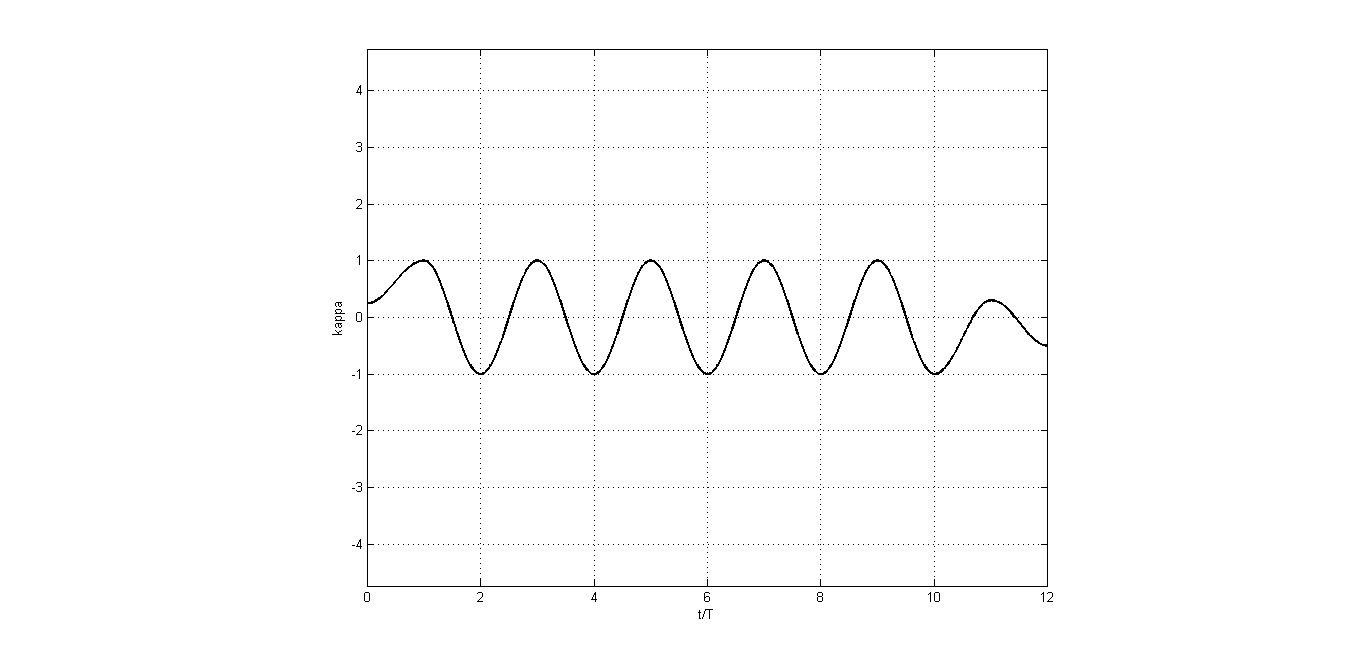
\includegraphics[width=160mm]{kappa}}
\caption{Пример закона изменения угла $\kappa$ во время поворота}
\label{controlsignal}
\end{figure}

Закон изменения строится в следующем порядке:

- по начальному положению модуля находим начальное положение $\kappa^0$


- в зависимости от направления разворота аппарата, какая нога находится в опоре и на какой опорной окружности, угол $\kappa$ из начального положения выводится в свое минимальное или максимальное возможное


- колебания угла $\kappa$ между минимальным и максимальным допустимыми значениями до тех пор пока одна из конечных следовых точек (рис. \ref{stepcase}) модуля не окажется в области достижимости очередного поперечного шага с максимальной длиной

- выполняется дошагивание в один или два шага для приведения Н-модуля и корпуса в требуемые конечные ориентации



Пример закона изменения угла $\kappa$ для случая (2,2) представлен на рис. \ref{controlsignal}. Законы изменения координат $d_l,d_r$ находятся по формулам (\ref{dldrsolution}).

%\subsection{Совместное движение Н-модулей}

Рассмотрим совместное движение двух Н-модулей. Как согласуются между собой углы $\kappa_1$ и $\kappa_2$ двух модулей? Пусть в начальный момент времени модули ориентированы вдоль корпуса аппарата, ноги расставлены как показано на рис. \ref{ortho_kinogramma}. Найдем связь между углами ориентации модулей $\phi_{11}$ и $\phi_{12}$.

Центр правого Н-модуля имеет координаты

$$
\left\{
\begin{array}{lcr}
x_1 = R\cos{\alpha}\\
y_1 = R\sin{\alpha}\\
\end{array}
\right.
$$

Координаты опорной точки правого Н-модуля

$$
\left\{
\begin{array}{lcr}
x_R = (R-r)\cos{\gamma_R}\\
y_R = (R-r)\sin{\gamma_R}\\
\end{array}
\right.
$$

где $\gamma_R$ определяет положение опорной точки для правого Н-модуля. Тогда, из условия отрицательности $d_1$ и того, что для правого Н-модуля опорной является левая нога, получаем:

$$
\left\{
\begin{array}{lcr}
d_{11} = -\sqrt{(x_R-x_{11})^2+(y_R-y_{11})^2-c^2}\\
\phi_{11} = \arctan\left(\dfrac{y_R-y_{11}}{x_R-x_{11}}\right)+arcsin{\left(\dfrac{c}{\sqrt{(y_R-y_{11})^2+(x_R-x_{11})^2}}\right)}\\
\end{array}
\right.
$$

аналогично для левого Н-модуля получаем:

$$
\left\{
\begin{array}{lcr}
d_{12} = -\sqrt{(x_L-x_{12})^2+(y_L-y_{12})^2-c^2}\\
\phi_{12} = \arctan\left(\dfrac{y_L-y_{12}}{x_L-x_{12}}\right)-arcsin{\left(\dfrac{c}{\sqrt{(y_L-y_{12})^2+(x_L-x_{12})^2}}\right)}\\
\end{array}
\right.
$$

Найденные углы $\phi_{11}$ и $\phi_{12}$ это абсолютные углы ориентации Н-модулей. Разница $\delta_\phi = \phi_{11}-\phi_{12}$ величина непостоянная и зависит от расположения опорных точек и ориентаций Н-модулей. При совместном синтезе законов изменения углов $\kappa_{ij}$ для Н-модулей при развороте аппарата нужно учитывать разницу рассогласование между правым и левым модулем. Остальные Н-модули выполняют симметричные движения в соответствии с центральной симметрией, т.е. правый задний Н-модуль копирует движение левого переднего Н-модуля, а левый задний Н-модуль копирует правый передний Н-модуль.

Рассогласование углов $\kappa_{ij}$ вызвано прямоугольной формой корпуса аппарата и зависит от того с какой ноги выполняется шаг. При квадратом корпусе все поворотные модули будут работать без рассогласования по абсолютным величинам углов $\kappa_{ij}$, а значит для робота с квадратным корпусом проще построить управление чем для прямоугольного.

Можно увидеть некоторую аналогию с кинематикой рулевой системы легковых автомобилей. При повороте, передние колеса автомобиля поворачиваются на разные углы для избежания проскальзывания колес в точках контакта. Роль колес в роботе с ортогональными движителями выполняют Н-модули.

\subsection{Моделирование}

Моделирование выполнялось в программном комплексе Универсальный Механизм (ПК УМ). В терминах этого программного комплекса механическая система рассматривается как система твердых тел. Взаимодействие тел задается при помощи различных шарниров и контактных сил. Уравнения движения синтезируются автоматически в символьном виде. После синтеза уравнений движения динамическая модель готова к запуску. ПК УМ имеет целый набор встроенных моделей контакта. Для простоты был выбран точечный контакт с вязко-упругой моделью взаимодействия.

\begin{figure}[h]
\center{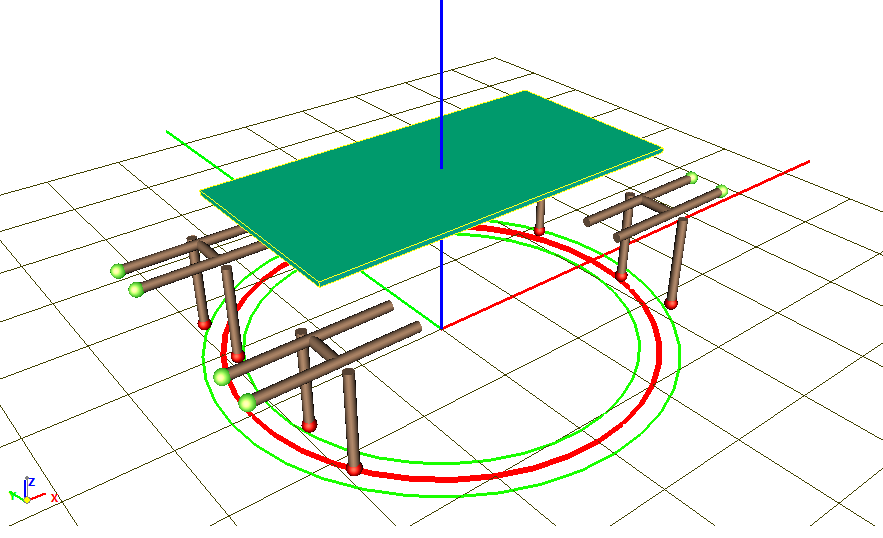
\includegraphics[width=100mm]{ortho_model}}
\caption{Общий вид модели аппарата}
\end{figure}

В шарнирах модели запрограммированы модели сервоприводов. Шарнирный момент или сила вычисляются при помощи PD регулятора:

$$
M = -\chi_1\,(x-x_p)-\chi_2\,\dot{x},
$$

где $M$ - управляющий шарнирный момент, $\chi_1>0$ и $\chi_2>0$ --- коэффициенты усиления, $x_p = x_p(t)$ --- программное значение шарнирной координаты, $x$ и $\dot{x}$ --- реализовавшиеся значение и скорость. Коэффициенты $\chi_1$ и $\chi_2$ выбираются так, чтобы рассогласование реального и программных значений уменьшалось экспоненциально быстро и без перерегулирования.

В файле управления модели запрограммированы все необходимые функции для решения задач кинематики, например, таких как расчет угла ориентации Н-модуля при повороте корпуса по заданным следовым точкам, расчет значений $d_l, d_r$ по углу $\kappa$ и остальное. На рис. \ref{ortho_kinogramma} представлена кинограмма движения аппарата во время моделирования. Снимки сделаны в моменты смены опорных ног.

\begin{figure}
\center{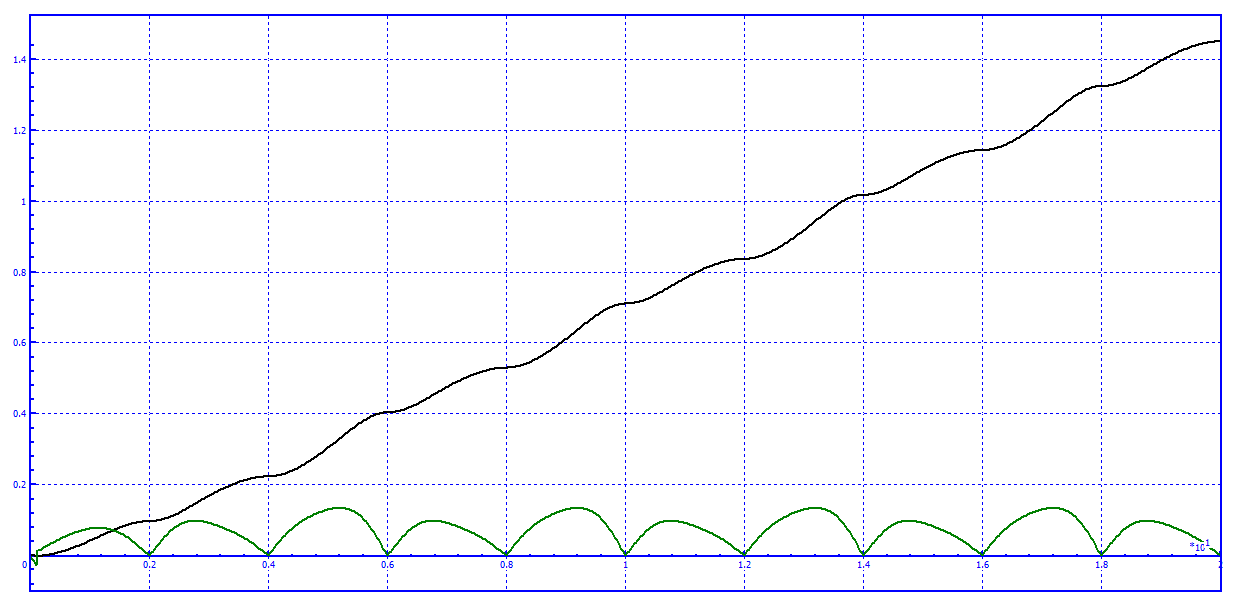
\includegraphics[width=120mm]{ortho_model5}}
\caption{График угла ориентации корпуса и угловая скорость корпуса}
\end{figure}



\begin{figure}
\begin{minipage}[h]{0.4\linewidth}
\center{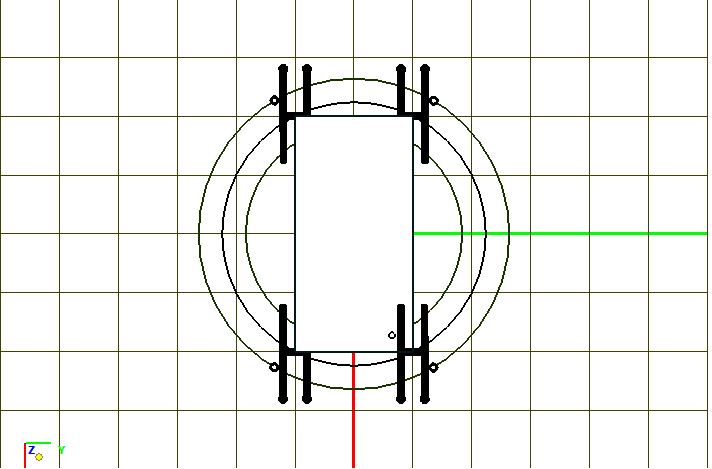
\includegraphics[width=1\linewidth]{ortho_model1}} 1) $t=0$ с\\
\end{minipage}
%\hfill
\begin{minipage}[h]{0.4\linewidth}
\center{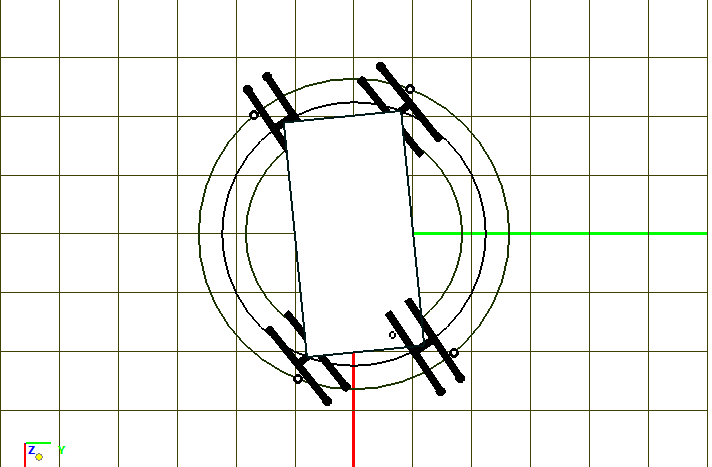
\includegraphics[width=1\linewidth]{ortho_model2}} 2) $t=2$ с\\
\end{minipage}
\begin{minipage}[h]{0.4\linewidth}
\center{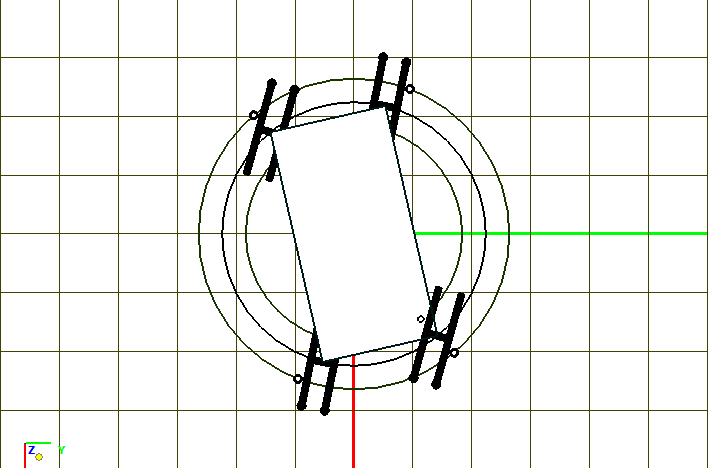
\includegraphics[width=1\linewidth]{ortho_model3}} 3) $t=4$ с\\
\end{minipage}
%\hfill
\begin{minipage}[h]{0.4\linewidth}
\center{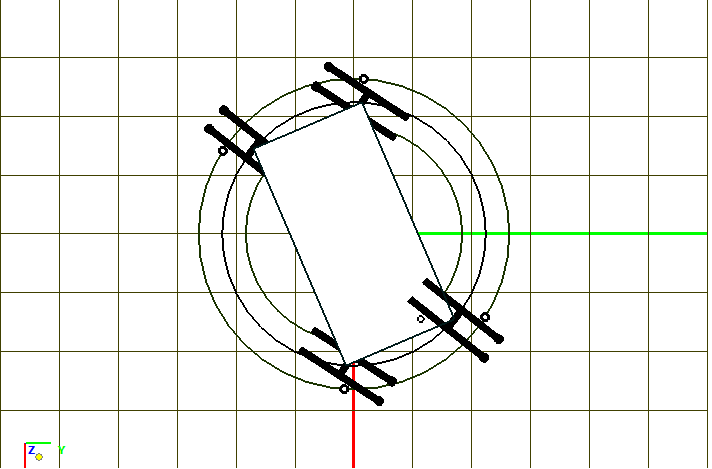
\includegraphics[width=1\linewidth]{ortho_model4}} 4) $t=6$ с\\
\end{minipage}
\begin{minipage}[h]{0.4\linewidth}
\center{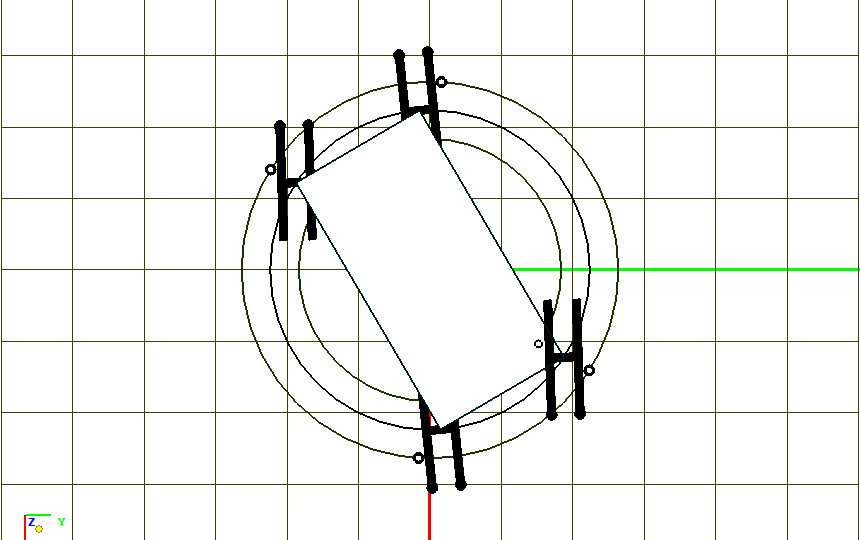
\includegraphics[width=1\linewidth]{ortho_model10}} 5) $t=8$ с\\
\end{minipage}
%\hfill
\begin{minipage}[h]{0.4\linewidth}
\center{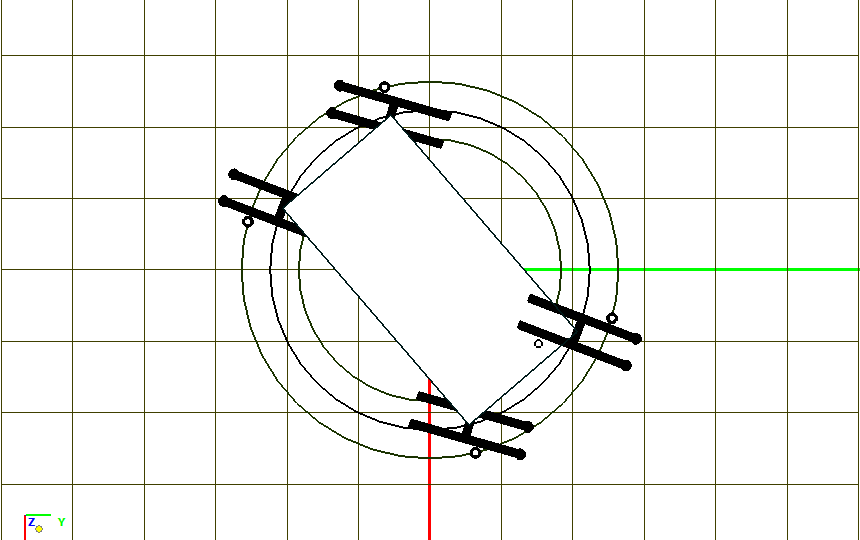
\includegraphics[width=1\linewidth]{ortho_model11}} 6) $t=10$ с\\
\end{minipage}
\begin{minipage}[h]{0.4\linewidth}
\center{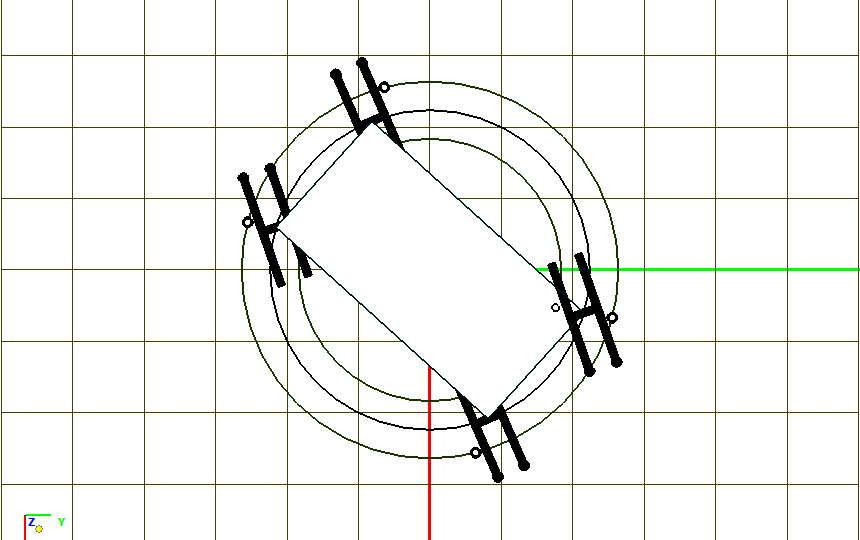
\includegraphics[width=1\linewidth]{ortho_model12}} 7) $t=12$ с\\
\end{minipage}
\hfill
\begin{minipage}[h]{0.4\linewidth}
\center{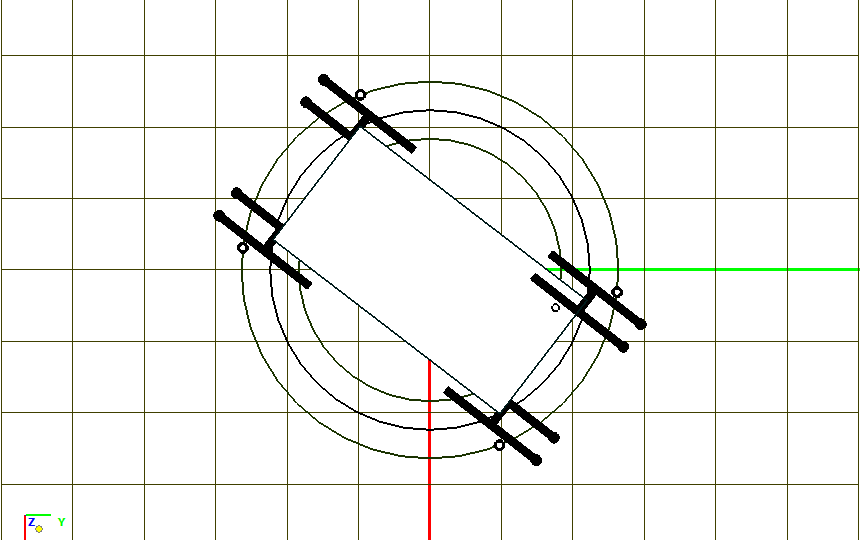
\includegraphics[width=1\linewidth]{ortho_model13}} 8) $t=13$ с\\
\end{minipage}
\caption{Кинограмма поворота аппарата. Вид сверху}
\label{ortho_kinogramma}
\end{figure}



%График изменения угла $\kappa$ и соответствующих переменных $d_l$ и $d_r$:

\begin{figure}
\center{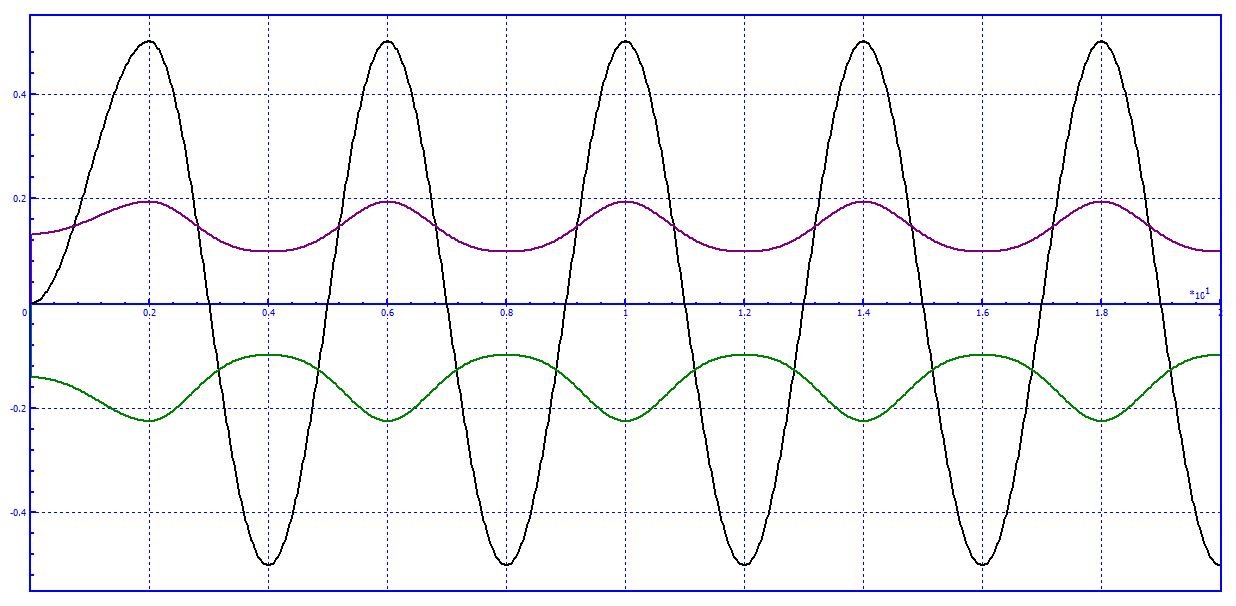
\includegraphics[width=120mm]{ortho_model6}}
\caption{График изменения угла $\kappa$ и переменных $d_l>0$ и $d_r<0$}
\end{figure}

\begin{figure}
\center{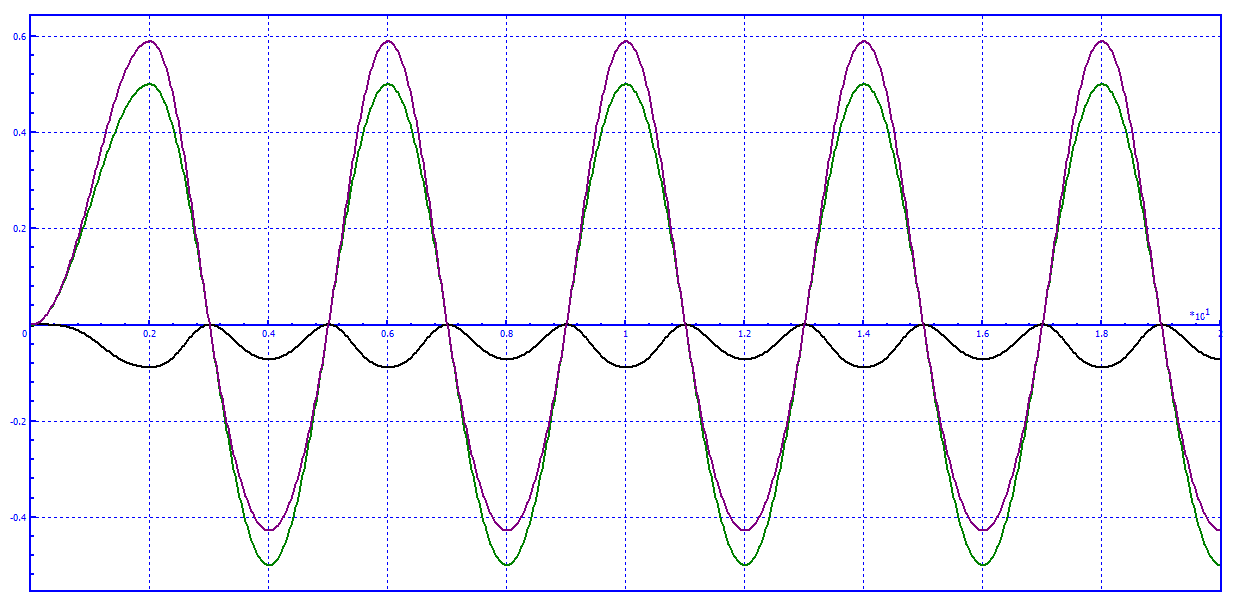
\includegraphics[width=120mm]{ortho_model14}}
\caption{Углы ориентации $\phi_1,\phi_2$  двух соседних Н-модулей и график $\delta_\phi$ рассогласования ориентации}
\end{figure}

\begin{figure}
\center{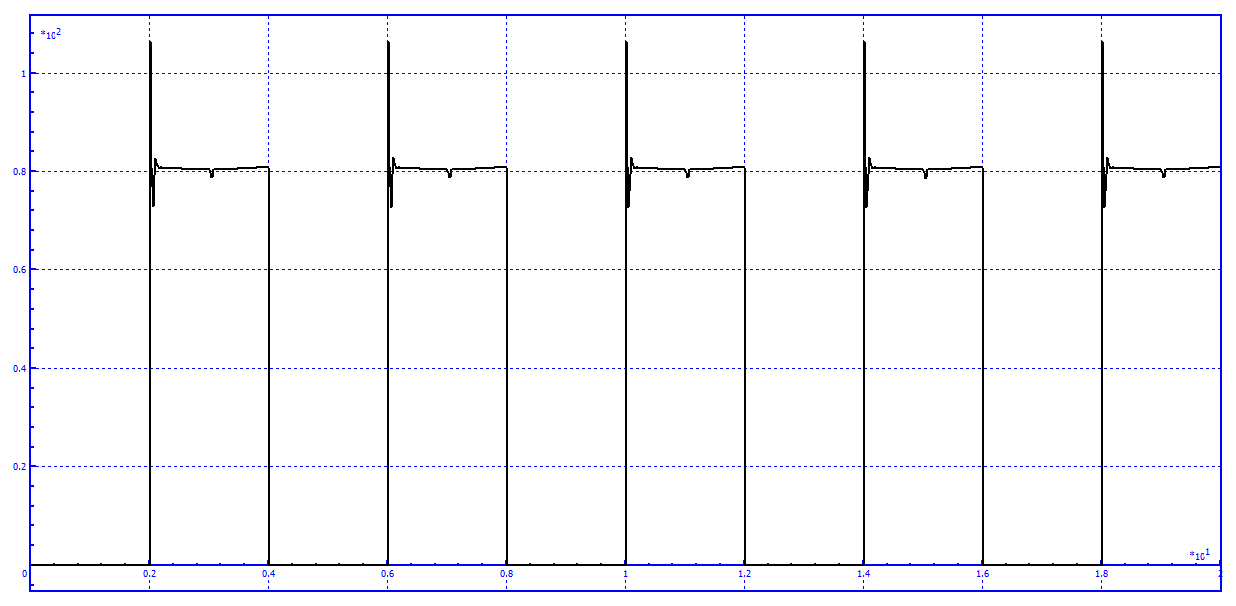
\includegraphics[width=120mm]{ortho_model7}}
\caption{Модуль реакции опоры для одной из ног}
\end{figure}

\begin{figure}
\center{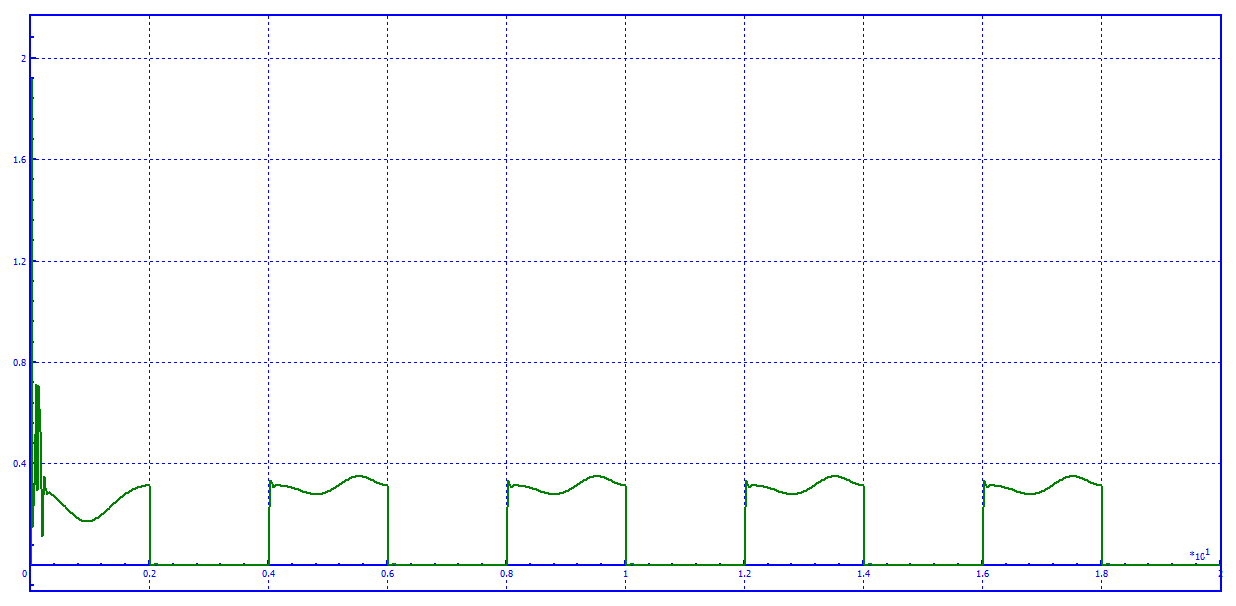
\includegraphics[width=120mm]{ortho_model8}}
\caption{Модуль абсолютной скорости контактной точки одной из ног}
\end{figure}

По графику абсолютной скорости контактной точки одной из ног можно заметить, что в опорной фазе скорость контактной точки равна нулю, а это значит, что все вычисления верны и разворот аппарата выполняется кинематически точно и без проскальзывания.

\begin{figure}
\center{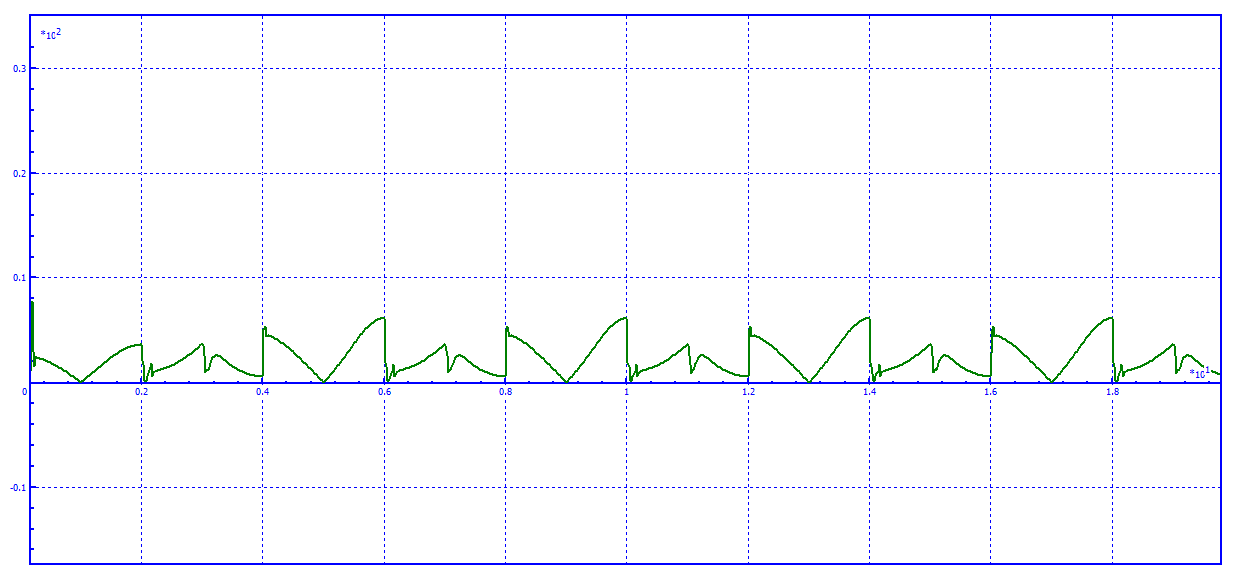
\includegraphics[width=120mm]{ortho_model9}}
\caption{Управляющий шарнирный момент Н-модуля}
\end{figure}


%%%%%%%%%%%%%%%%%%%%%%%%%%%%%%%%
%\chapter{Оформление различных элементов} \label{chapt1}
%
%\section{Форматирование текста} \label{sect1_1}
%
%Мы можем сделать \textbf{жирный текст} и \textit{курсив}.
%
%%\newpage
%%============================================================================================================================
%
%\section{Ссылки} \label{sect1_2}
%Сошлемся на библиографию: \cite{bib1}, \cite{bib2}, \cite{bib3,bib4,bib5}.
%
%Сошлемся на приложения: Приложение \ref{AppendixA}, Приложение \ref{AppendixB2}.
%
%Сошлемся на формулу: формула (\ref{eq:equation1}).
%
%Сошлемся на изображение: рисунок \ref{img:knuth}.
%
%%\newpage
%%============================================================================================================================
%
%\section{Формулы} \label{sect1_3}
%
%\subsection{Ненумерованные одиночные формулы} \label{subsect1_3_1}
%
%Вот так может выглядеть формула, которую необходимо вставить в строку по тексту: $x \approx \sin x$ при $x \to 0$.
%
%А вот так выглядит ненумерованая отдельностоящая формула c подстрочными и надстрочными индексами:
%$$
%(x_1+x_2)^2 = x_1^2 + 2 x_1 x_2 + x_2^2
%$$
%
%При использовании дробей формулы могут получаться очень высокие:
%$$
%  \frac{1}{\sqrt(2)+
%  \displaystyle\frac{1}{\sqrt{2}+
%  \displaystyle\frac{1}{\sqrt{2}+\cdots}}}
%$$
%
%В формулах можно использовать греческие буквы:
%$$
%\alpha\beta\gamma\delta\epsilon\varepsilon\zeta\eta\theta\vartheta\iota\kappa\lambda\\mu\nu\xi\pi\varpi\rho\varrho\sigma\varsigma\tau\upsilon\phi\varphi\chi\psi\omega\Gamma\Delta\Theta\Lambda\Xi\Pi\Sigma\Upsilon\Phi\Psi\Omega
%$$
%
%%\newpage
%%============================================================================================================================
%
%\subsection{Ненумерованные многострочные формулы} \label{subsect1_3_2}
%
%Вот так можно написать две формулы, не нумеруя их, чтобы знаки равно были строго друг под другом:
%\begin{eqnarray}
%  f_W & = & \min \left( 1, \max \left( 0, \frac{W_{soil} / W_{max}}{W_{crit}} \right)  \right), \nonumber \\
%  f_T & = & \min \left( 1, \max \left( 0, \frac{T_s / T_{melt}}{T_{crit}} \right)  \right), \nonumber
%\end{eqnarray}
%
%Можно использовать разные математические алфавиты:
%\begin{eqnarray}
%\mathcal{ABCDEFGHIJKLMNOPQRSTUVWXYZ} \nonumber \\
%\mathfrak{ABCDEFGHIJKLMNOPQRSTUVWXYZ} \nonumber \\
%\mathbb{ABCDEFGHIJKLMNOPQRSTUVWXYZ} \nonumber
%\end{eqnarray}
%
%Посмотрим на систему уравнений на примере аттрактора Лоренца:
%
%$$
%\left\{
%  \begin{array}{rl}
%    \dot x = & \sigma (y-x) \\
%    \dot y = & x (r - z) - y \\
%    \dot z = & xy - bz
%  \end{array}
%\right.
%$$
%
%А для верстки матриц удобно использовать многоточия:
%$$
%\left(
%  \begin{array}{ccc}
%  	a_{11} & \ldots & a_{1n} \\
%  	\vdots & \ddots & \vdots \\
%  	a_{n1} & \ldots & a_{nn} \\
%  \end{array}
%\right)
%$$
%
%
%%\newpage
%%============================================================================================================================
%\subsection{Нумерованные формулы} \label{subsect1_3_3}
%
%А вот так пишется нумерованая формула:
%\begin{equation}
%  \label{eq:equation1}
%  e = \lim_{n \to \infty} \left( 1+\frac{1}{n} \right) ^n
%\end{equation}
%
%Нумерованых формул может быть несколько:
%\begin{equation}
%  \label{eq:equation2}
%  \lim_{n \to \infty} \sum_{k=1}^n \frac{1}{k^2} = \frac{\pi^2}{6}
%\end{equation}
%
%В последствии на формулы (\ref{eq:equation1}) и (\ref{eq:equation2}) можно ссылаться.
%
%%\newpage
%%============================================================================================================================
%
%\clearpage
